\documentclass[11pt,a4paper]{article}

\usepackage[margin=1in]{geometry}
\usepackage{graphicx}
\usepackage{xcolor}
\usepackage{titlesec}
\usepackage{enumitem}
\usepackage{hyperref}
\usepackage{fancyhdr}
\usepackage{float}

\definecolor{brandindigo}{HTML}{4F46E5}
\definecolor{brandamber}{HTML}{F59E0B}
\definecolor{brandgray}{HTML}{4B4B57}

\titleformat{\section}{\normalfont\Large\bfseries\color{brandindigo}}{\thesection}{1em}{}
\titleformat{\subsection}{\normalfont\large\bfseries\color{brandgray}}{\thesubsection}{1em}{}

\pagestyle{fancy}
\fancyhf{}
\fancyhead[L]{VenueLock User Guide}
\fancyhead[R]{\thepage}
\renewcommand{\headrulewidth}{0.4pt}

\hypersetup{
    colorlinks=true,
    linkcolor=brandindigo,
    urlcolor=brandindigo,
}

\title{\textbf{\Huge VenueLock} \\[0.3em] \Large Lock the headcount. Unlock smooth entry. \\[0.5em] \normalsize User Guide}
\author{}
\date{}

\begin{document}

\maketitle
\thispagestyle{empty}

\begin{center}

\includegraphics[width=0.28\textwidth]{screenshots/app_icon.png}
\end{center}

\newpage
\tableofcontents
\newpage

% ─────────────────────────────────────────────────────────────
\section{Introduction}

VenueLock caps event attendance at an exact seat count. An organizer creates
a venue with a fixed seat map, attendees book a specific seat with a short
join code, and every booking produces a QR entry pass that is scanned at the
door.

\begin{itemize}[leftmargin=1.5em]
    \item \textbf{No overbooking} --- seat capacity is enforced on the
        server, so two people can never hold the same seat.
    \item \textbf{No paper tickets} --- the QR entry pass lives on the
        attendee's phone and survives a restart.
    \item \textbf{No bottleneck at the gate} --- several approved
        volunteers can scan in parallel, each with their own access.
    \item \textbf{No spreadsheets} --- seat and check-in status update
        live on every device at the venue.
\end{itemize}

\subsection{The three roles}

One app serves three kinds of user, chosen from the first screen:

\begin{itemize}[leftmargin=1.5em]
    \item \textbf{Admin} --- creates and configures venues, reserves seats
        for guests, reviews volunteer applications, and scans at the door.
    \item \textbf{Audience} --- joins a venue with its code, books a seat,
        and carries the entry pass.
    \item \textbf{Volunteer} --- applies to one venue with its access code
        and, once approved, scans entry passes at the gate.
\end{itemize}

\begin{figure}[H]
    \centering
    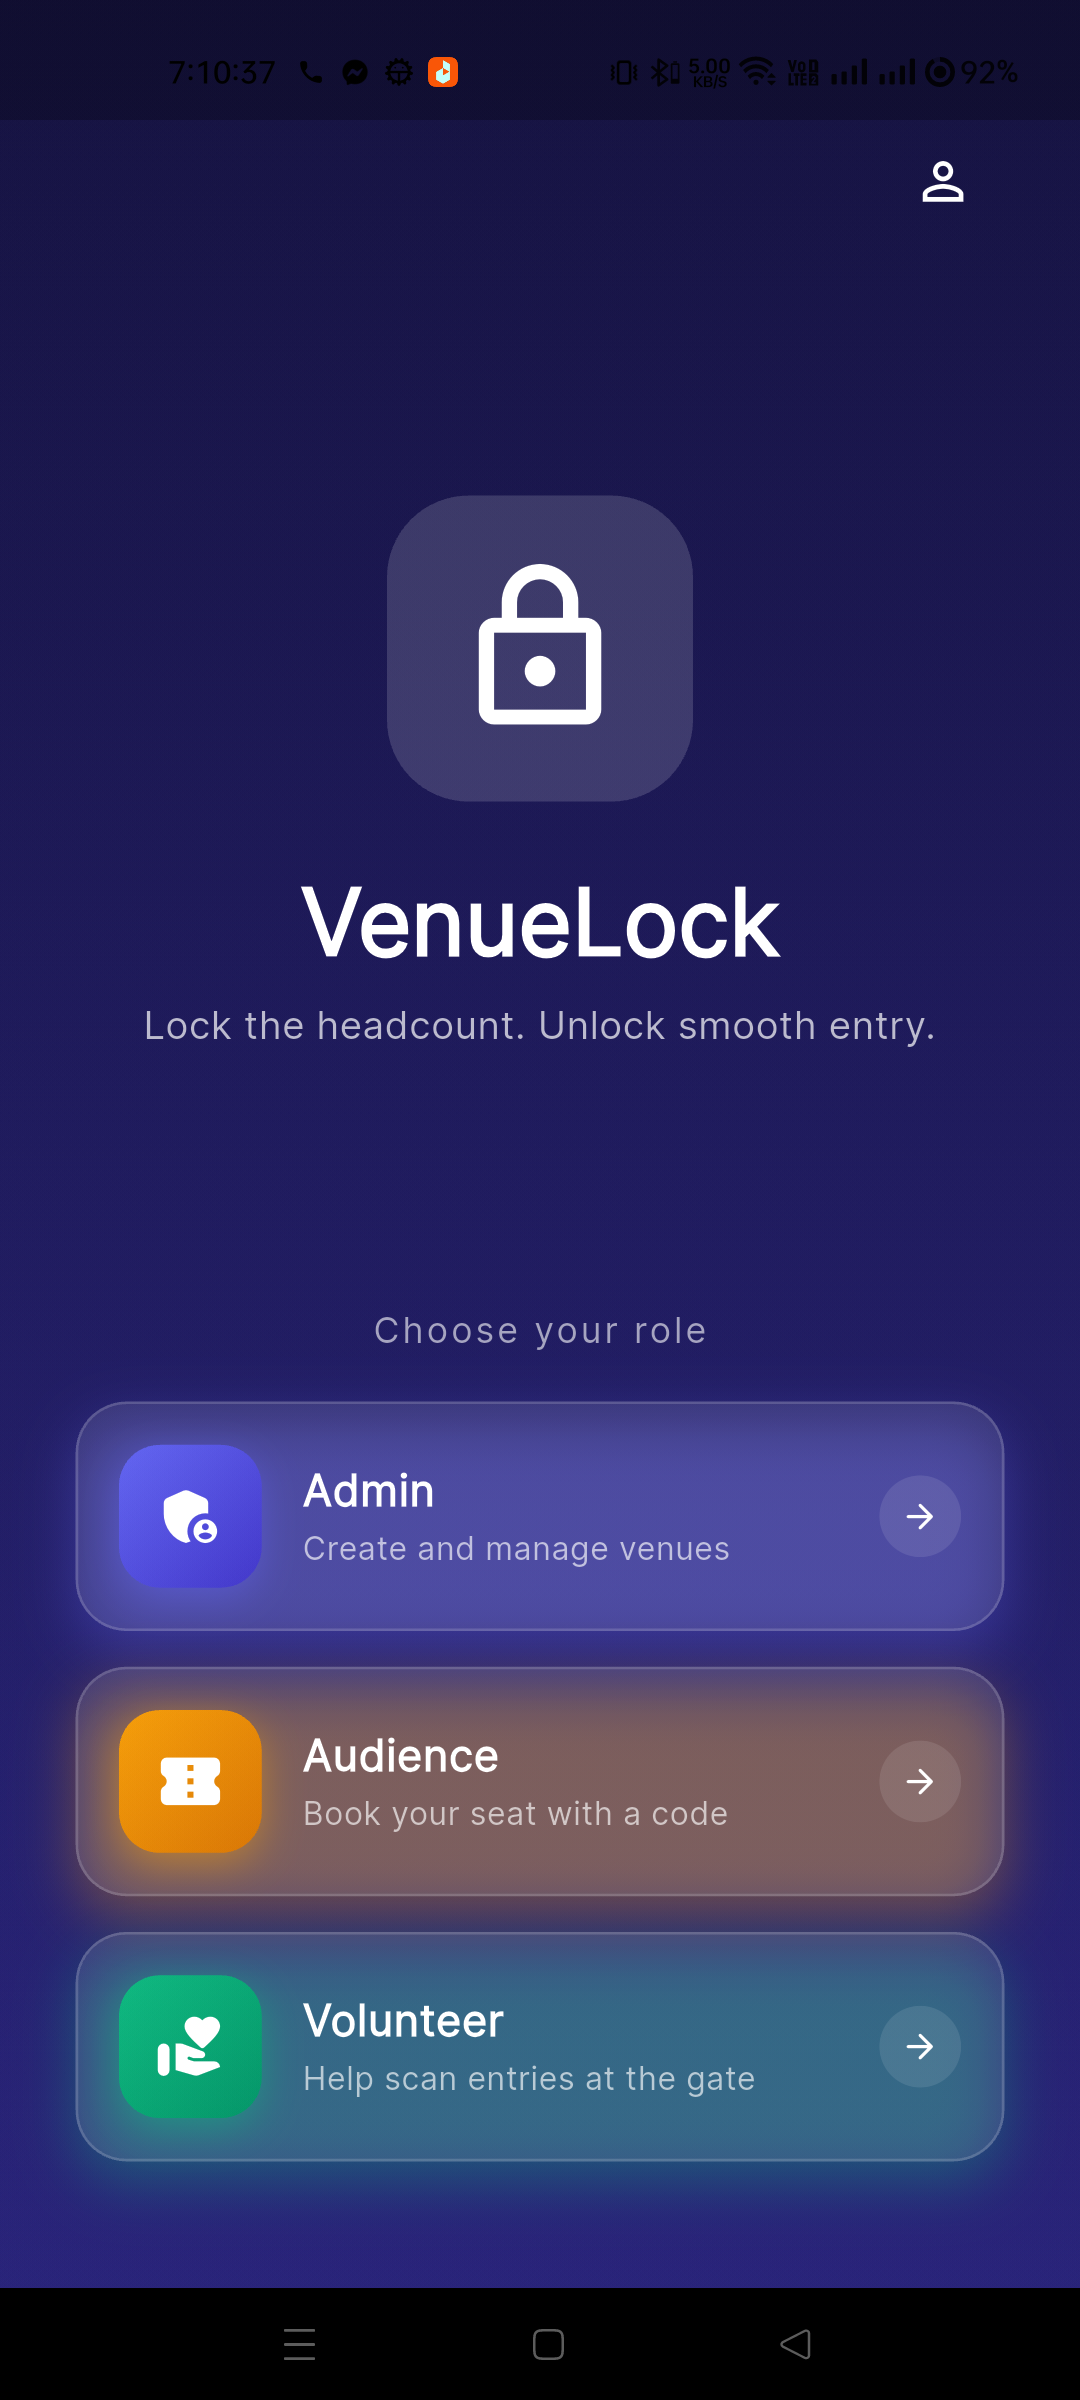
\includegraphics[width=0.42\textwidth]{screenshots/01_role_select.png}
    \caption{Choose your role when the app opens}
\end{figure}

% ─────────────────────────────────────────────────────────────
\section{Your Profile}

The person icon in the top-right corner of the role screen opens
\textbf{My Profile}. The name, email, and roll number saved here are used to
prefill booking and volunteer forms on this device, so attendees do not have
to retype them for every event. The same screen lists shortcuts to the Admin
Console, your Entry Passes, and your Volunteering activity.

\begin{figure}[H]
    \centering
    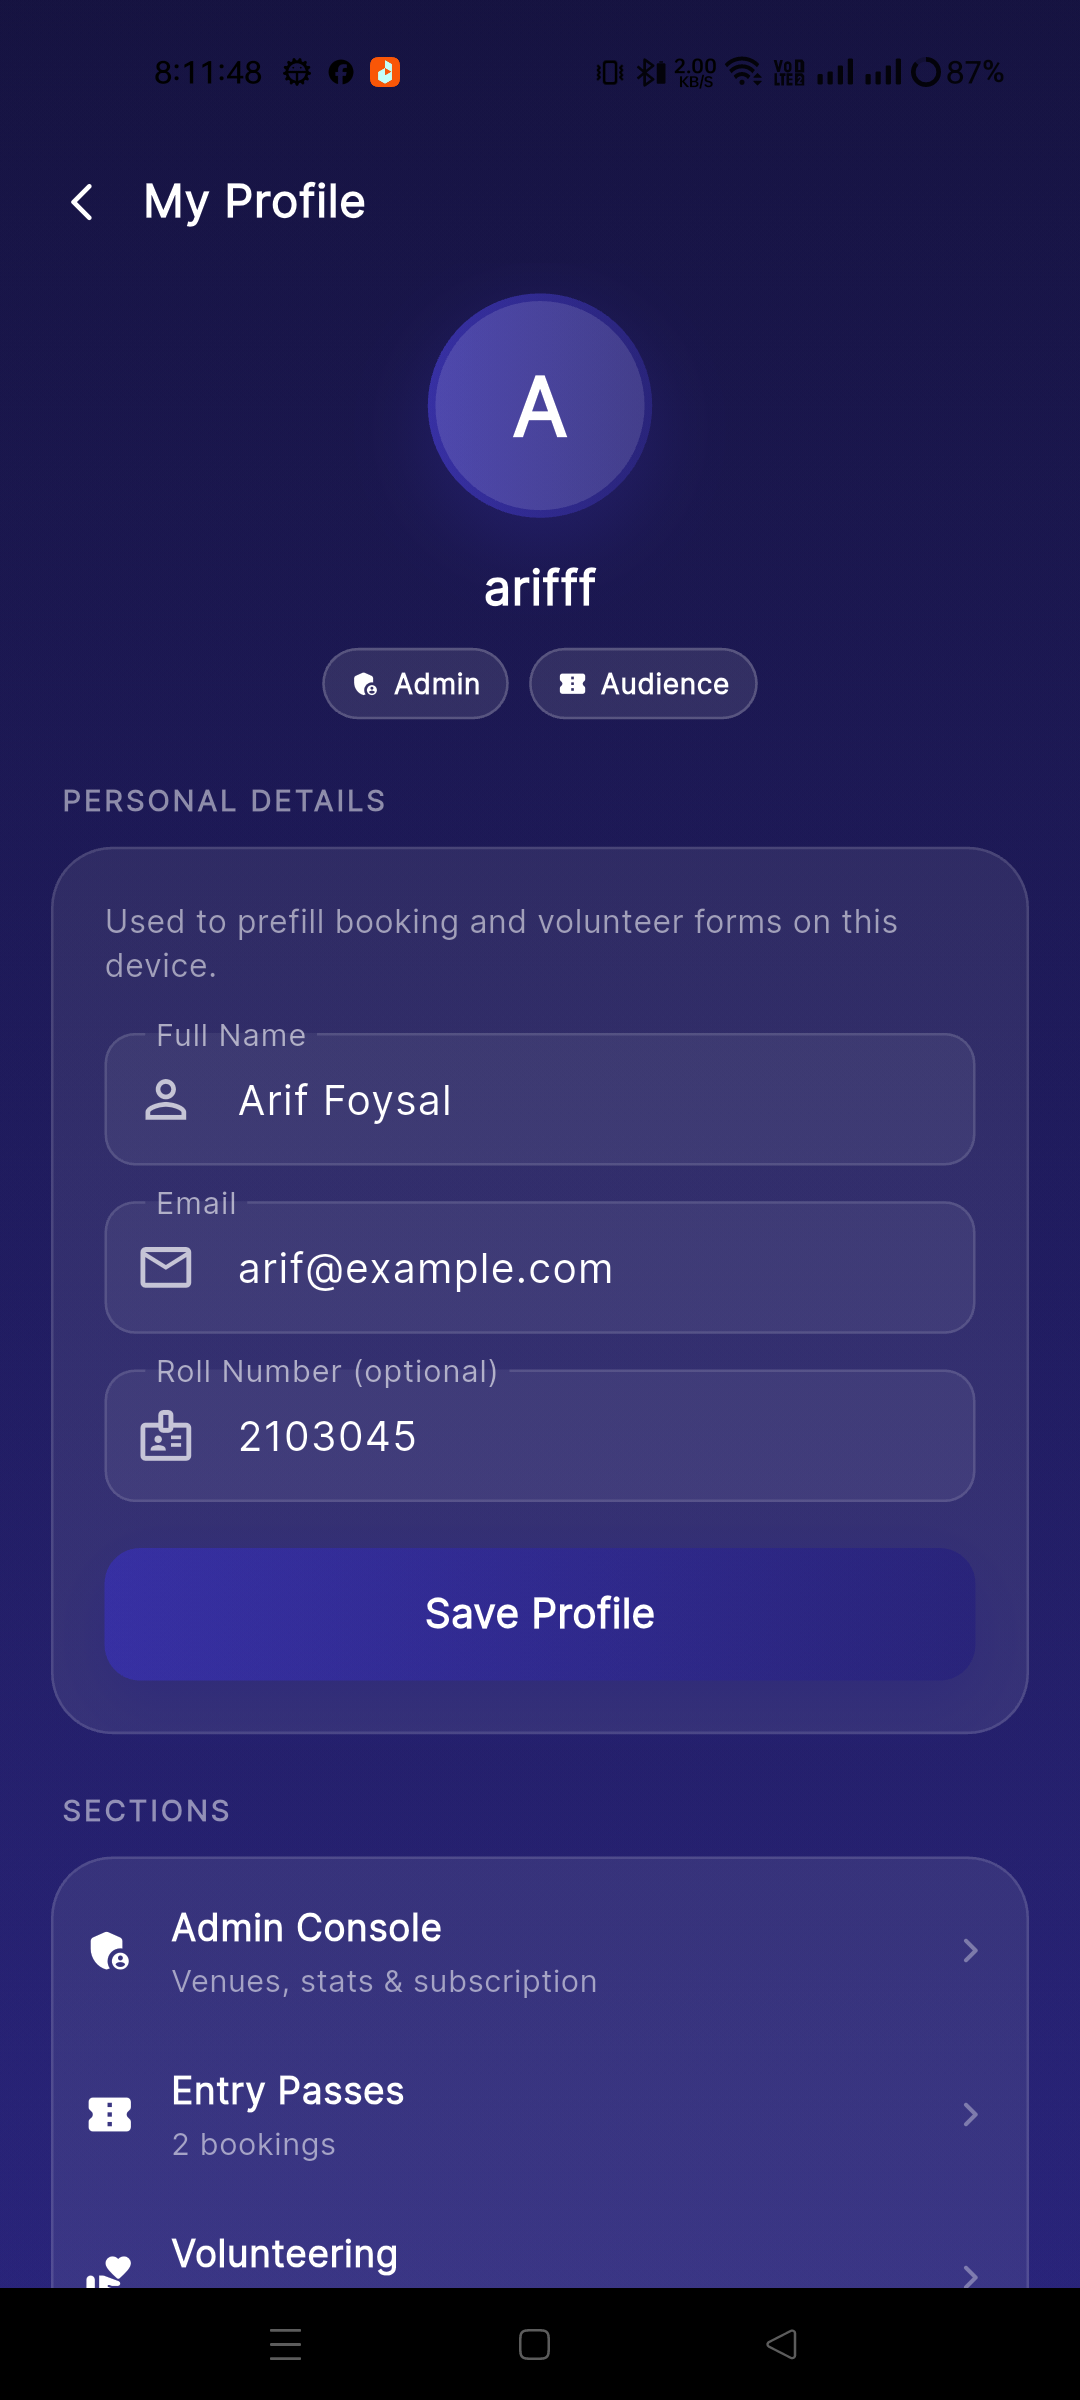
\includegraphics[width=0.42\textwidth]{screenshots/17_profile.png}
    \caption{My Profile --- personal details and role shortcuts}
\end{figure}

% ─────────────────────────────────────────────────────────────
\section{For Admins}

\subsection{The Admin Dashboard}

Choosing \textbf{Admin} opens your dashboard. The three tiles at the top
summarise every venue you own: how many venues you run, how many seats are
booked in total, and how many people have been checked in. Below them is one
card per venue, each showing its date, its sections, its booking progress
bar, and whether it is still \textbf{OPEN}.

\begin{figure}[H]
    \centering
    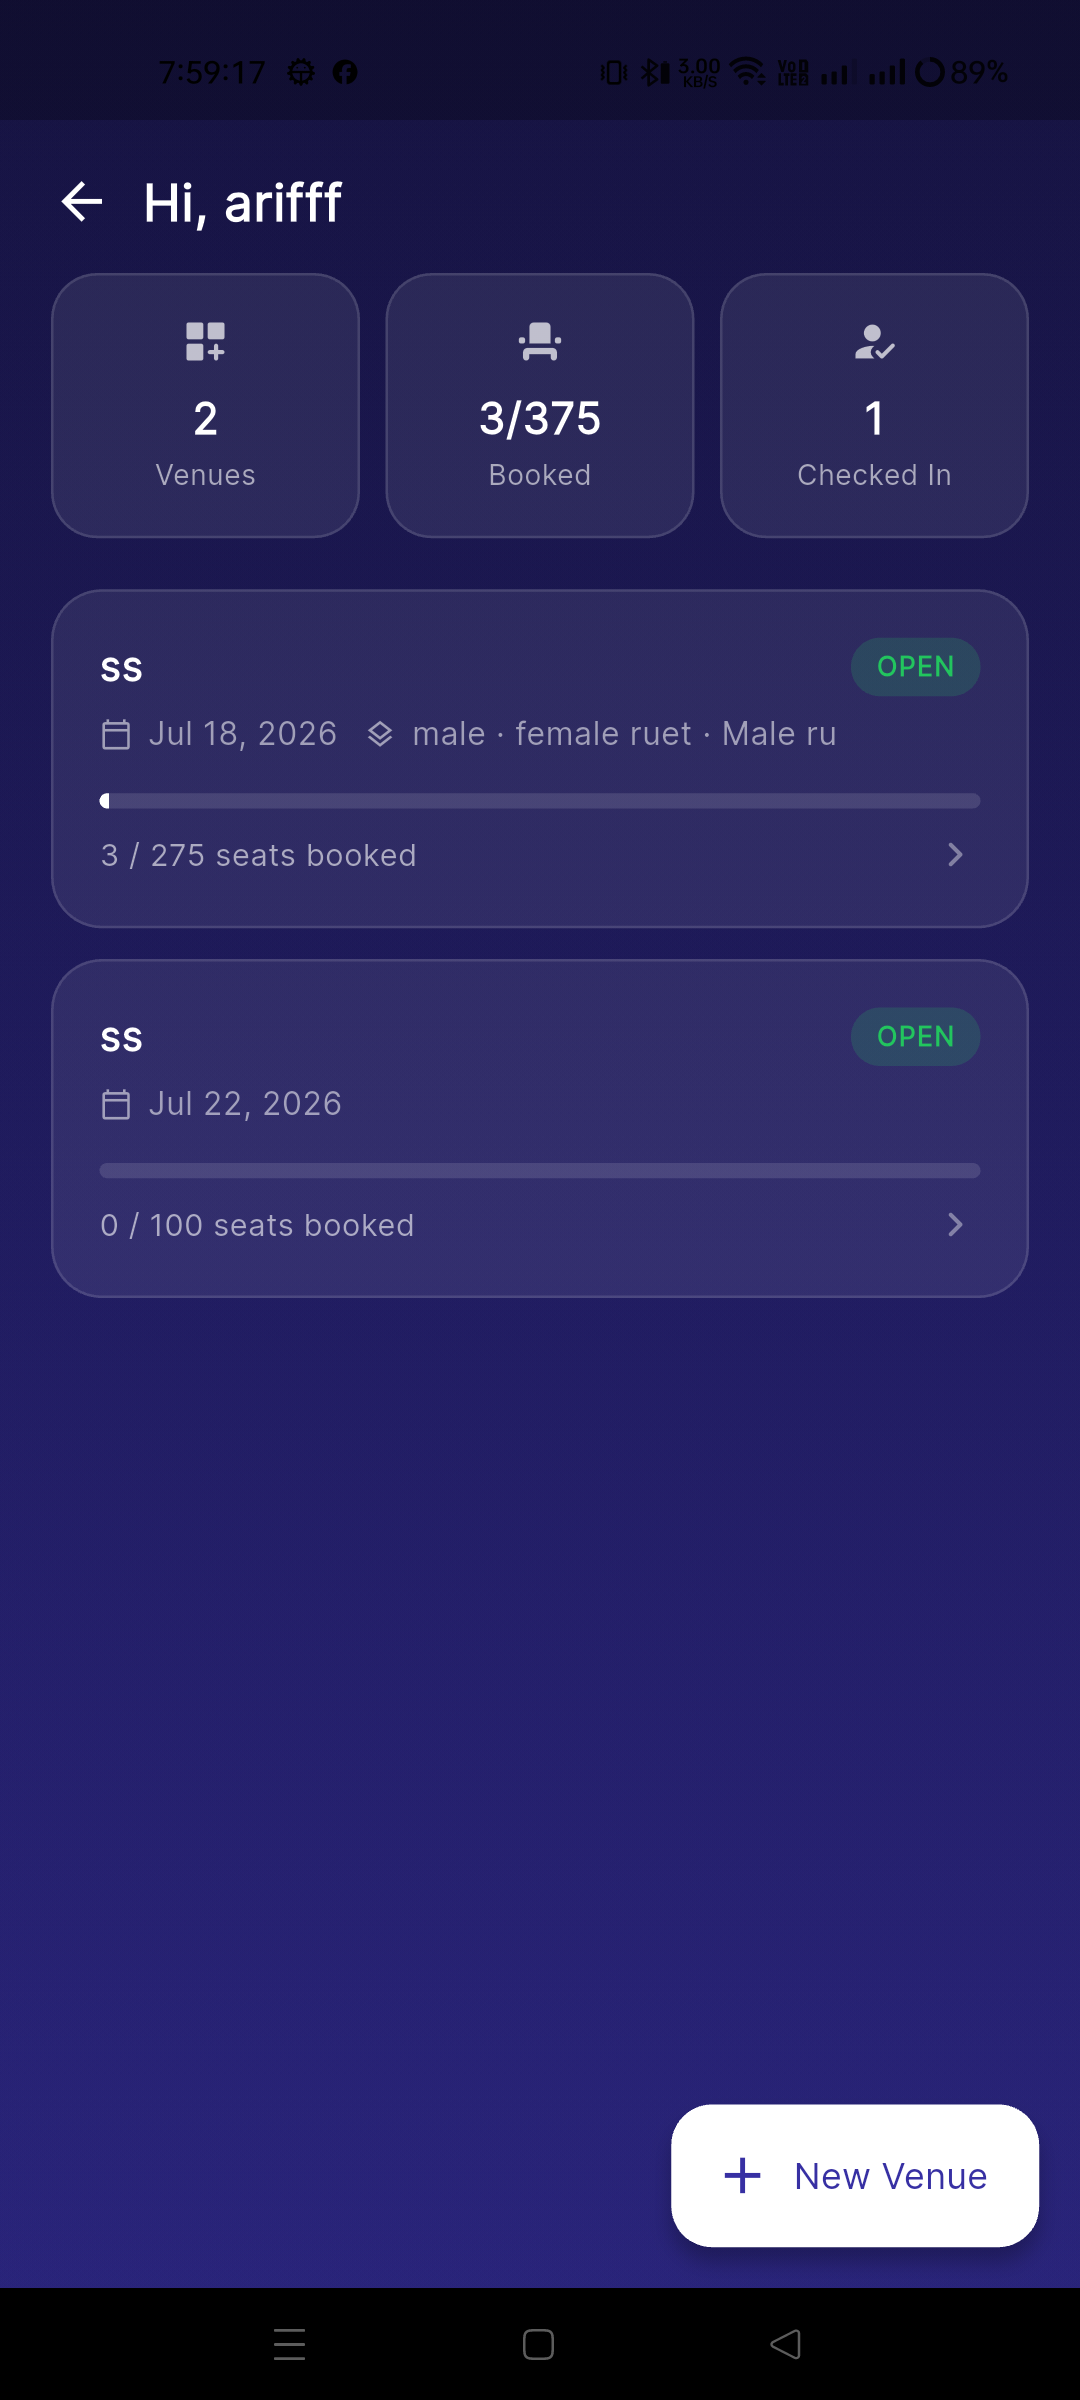
\includegraphics[width=0.42\textwidth]{screenshots/02_admin_dashboard.png}
    \caption{Admin dashboard with venue cards and live totals}
\end{figure}

\subsection{Creating a Venue}

Tap \textbf{+ New Venue}. Creation is a three-step wizard, tracked by the
dots at the top of the screen.

\paragraph{Step 1 --- Venue details.}
Give the venue a name and pick the event date.

\begin{figure}[H]
    \centering
    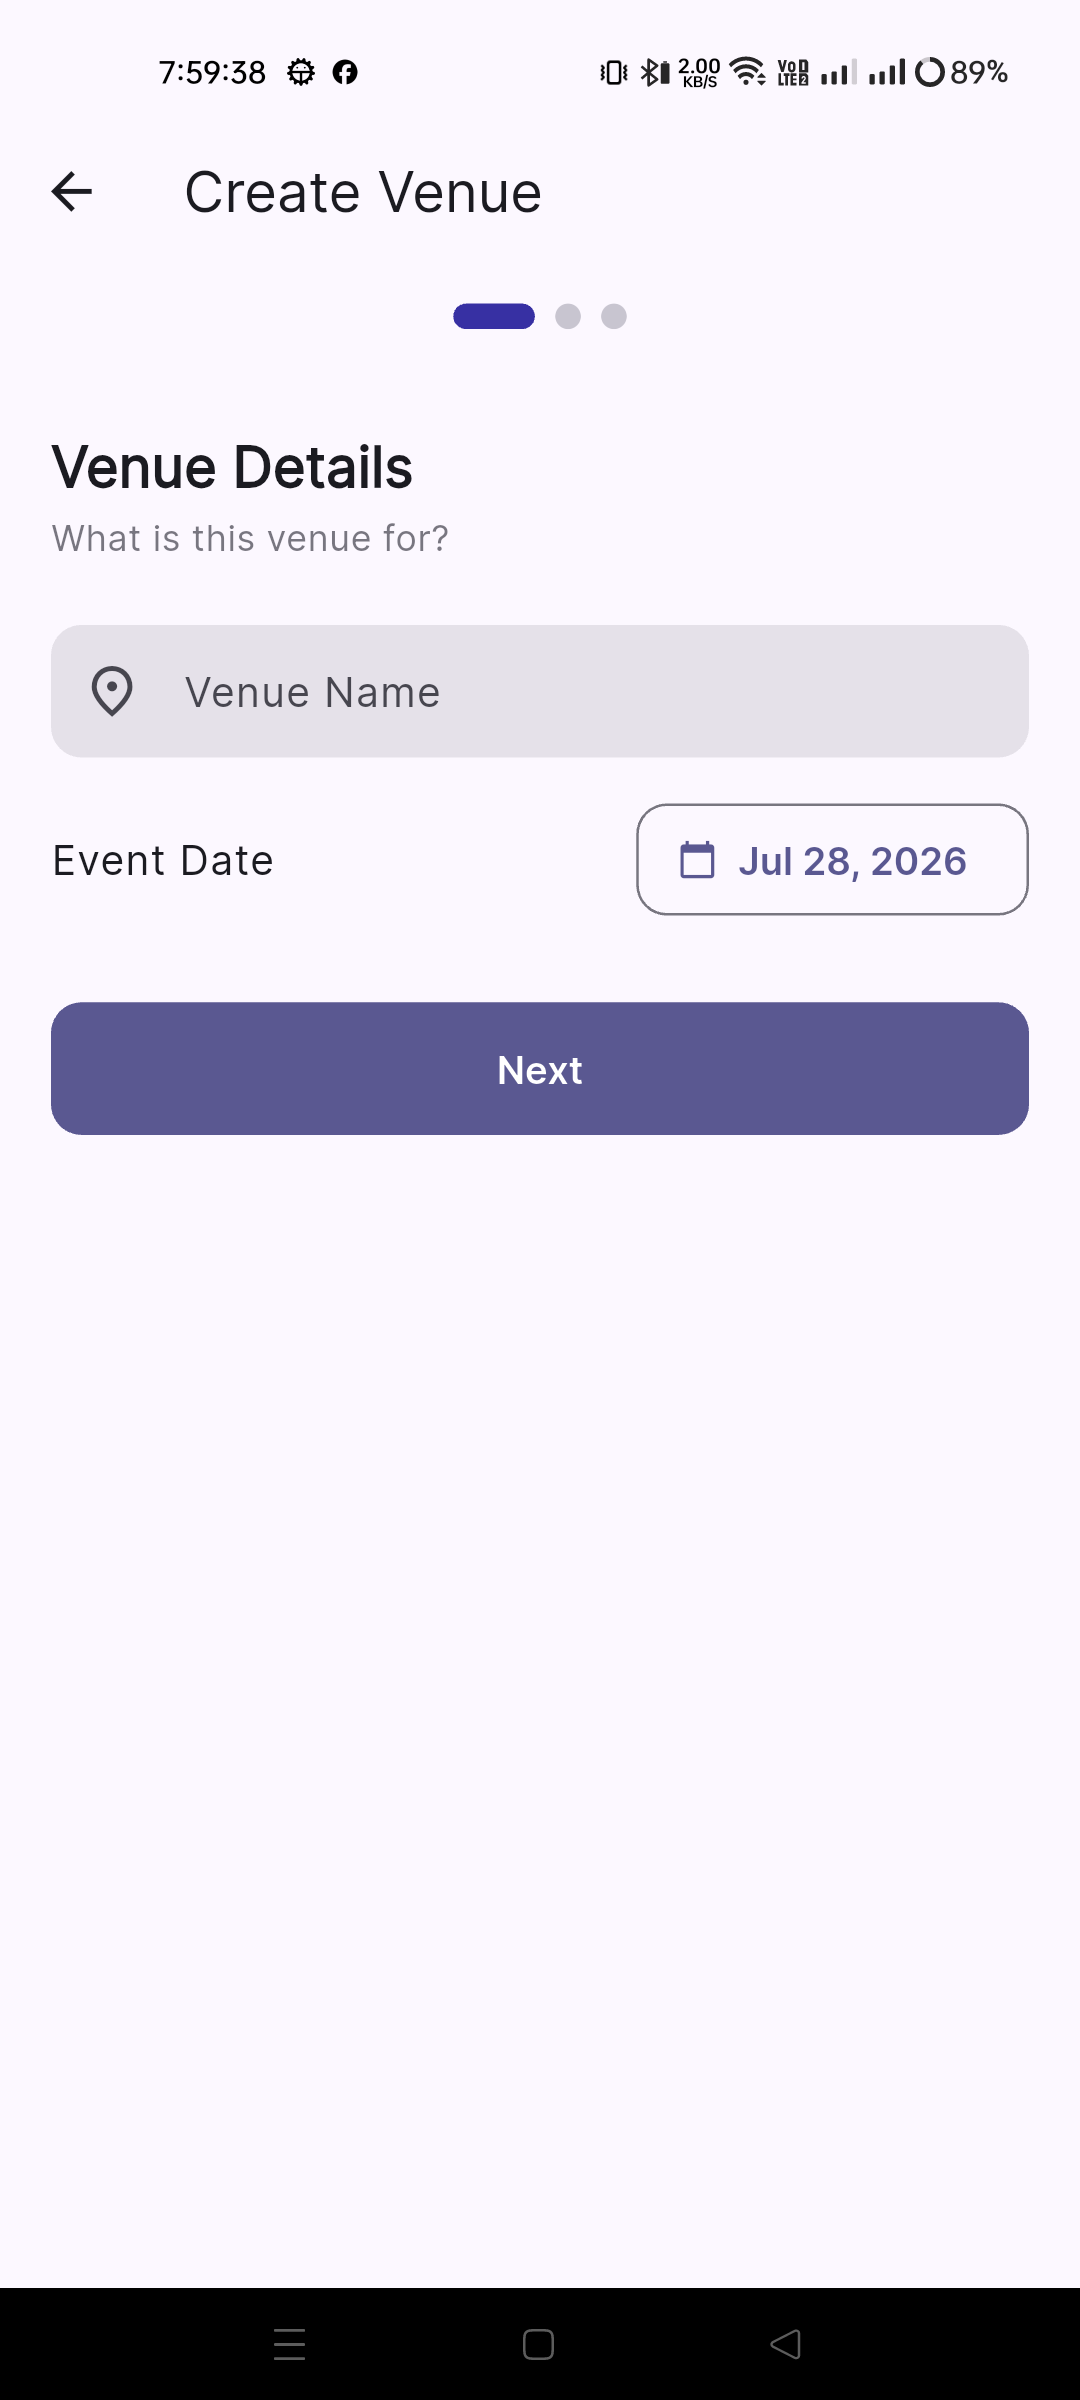
\includegraphics[width=0.42\textwidth]{screenshots/03_create_venue_details.png}
    \caption{Step 1 --- name and event date}
\end{figure}

\paragraph{Step 2 --- Seat layout.}
A venue is made of one or more \textbf{sections}. Each section has a name
and a grid of rows and columns; the running total at the top of the screen
tells you exactly how many seats the venue will hold. Use \textbf{+ Add
Section} for venues split into blocks (for example \textit{male},
\textit{female}, and a guest block), each with its own size.

\begin{figure}[H]
    \centering
    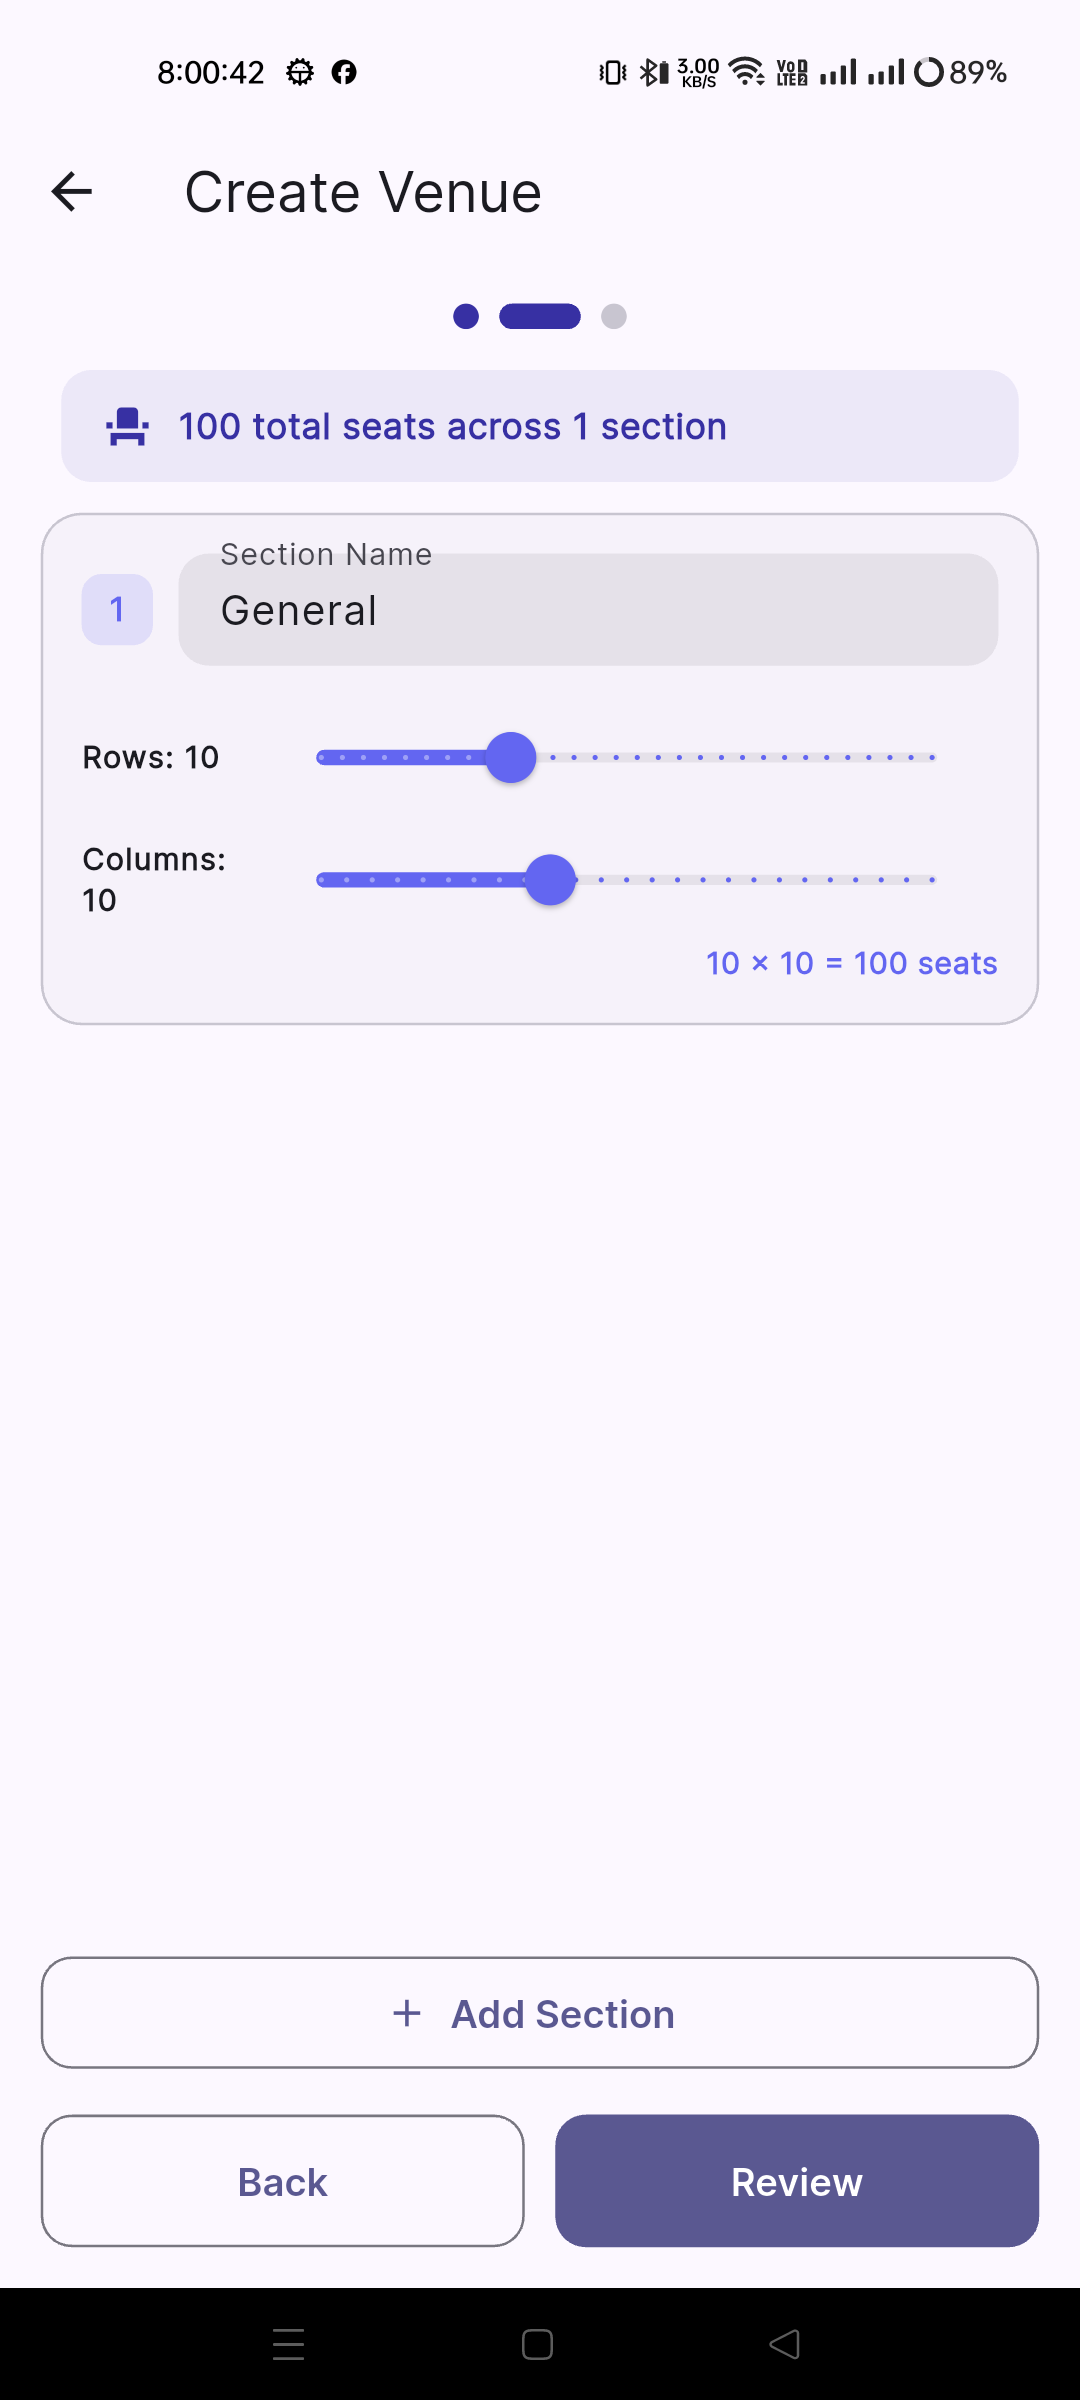
\includegraphics[width=0.42\textwidth]{screenshots/04_create_venue_sections.png}
    \caption{Step 2 --- sections, rows, and columns}
\end{figure}

\paragraph{Step 3 --- Review and publish.}
Check the summary and tap \textbf{Publish Venue}. The seat map is created on
the server at this point, and the venue's capacity is fixed.

\begin{figure}[H]
    \centering
    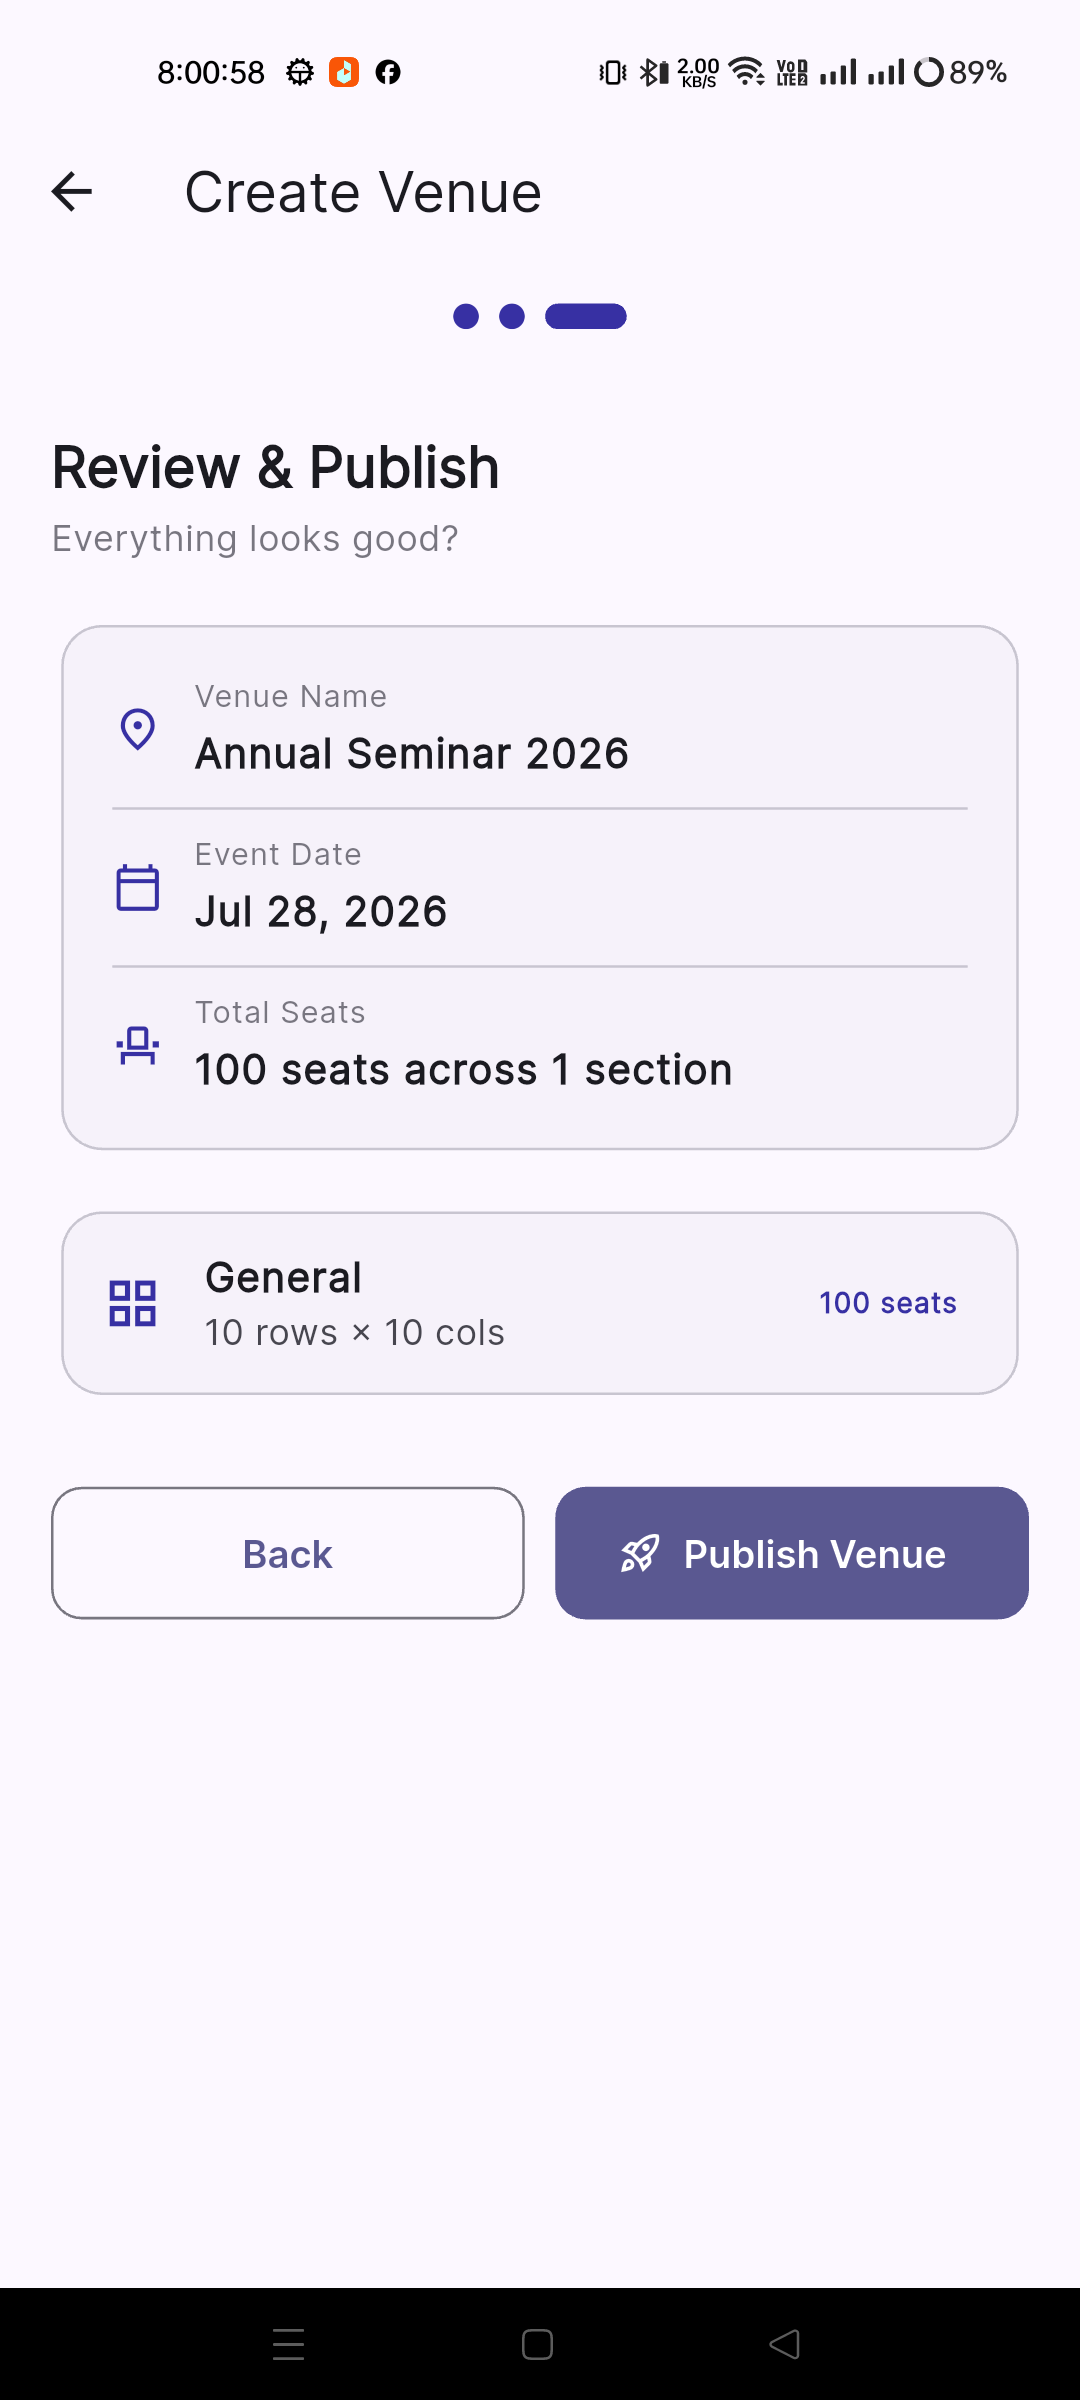
\includegraphics[width=0.42\textwidth]{screenshots/05_create_venue_review.png}
    \caption{Step 3 --- review and publish}
\end{figure}

\subsection{The Venue Screen and Access Code}

Publishing takes you straight to the venue screen. This is the control
centre for one event: live booked and checked-in counts, the section list,
the attendee list, and --- most importantly --- the six-character
\textbf{access code}.

Share that code with attendees so they can book a seat, and with volunteers
so they can apply to scan at this venue. The copy icon beside it puts the
code on the clipboard.

\begin{figure}[H]
    \centering
    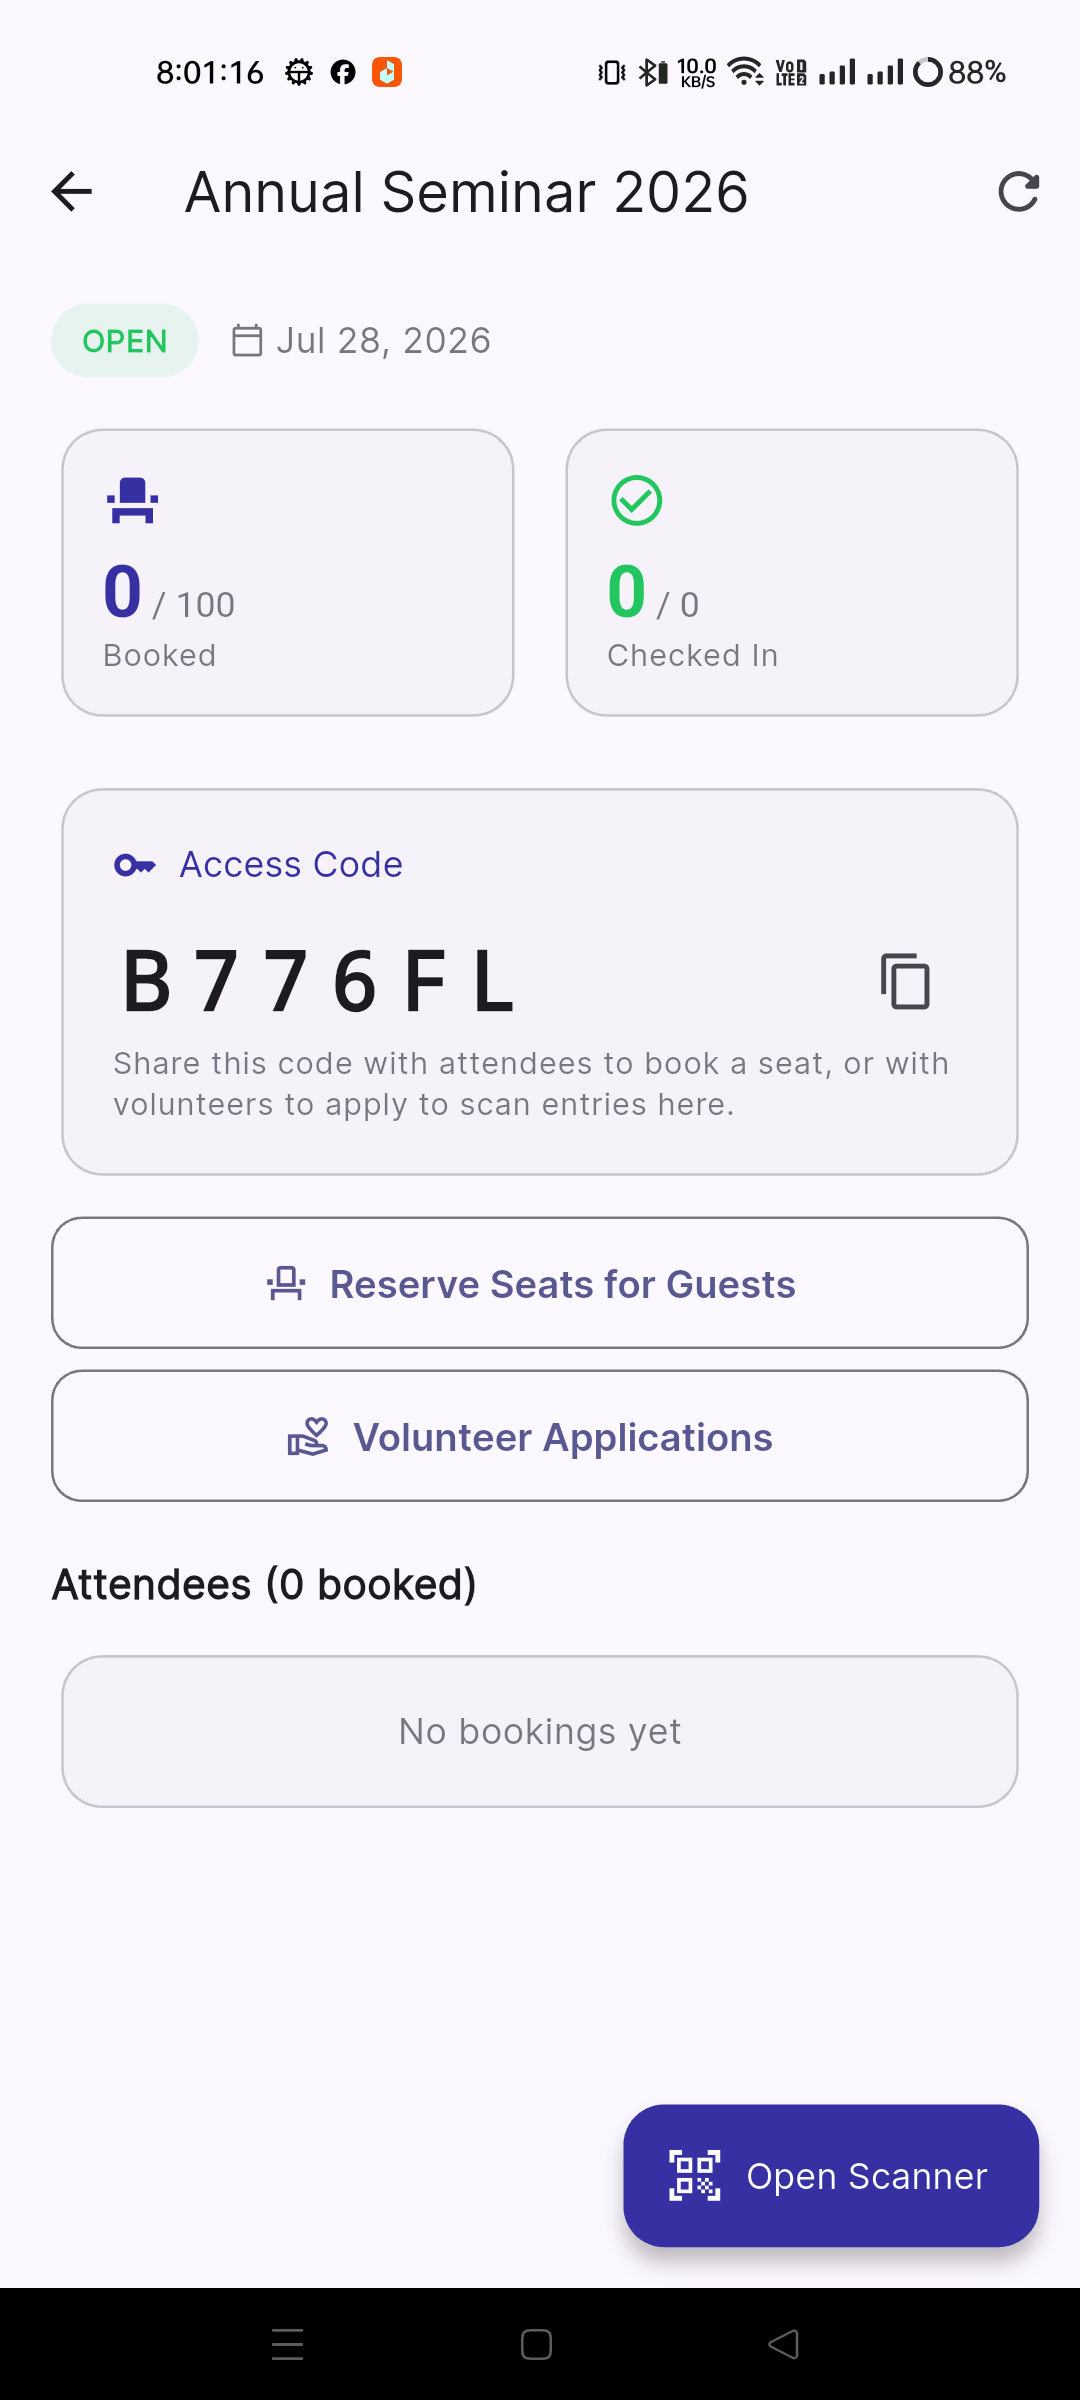
\includegraphics[width=0.42\textwidth]{screenshots/06_venue_detail.png}
    \caption{A freshly published venue and its access code}
\end{figure}

As bookings arrive, the same screen fills in: sections, attendee names with
their seat numbers, and a \textbf{Checked In} badge for everyone already
through the door.

\begin{figure}[H]
    \centering
    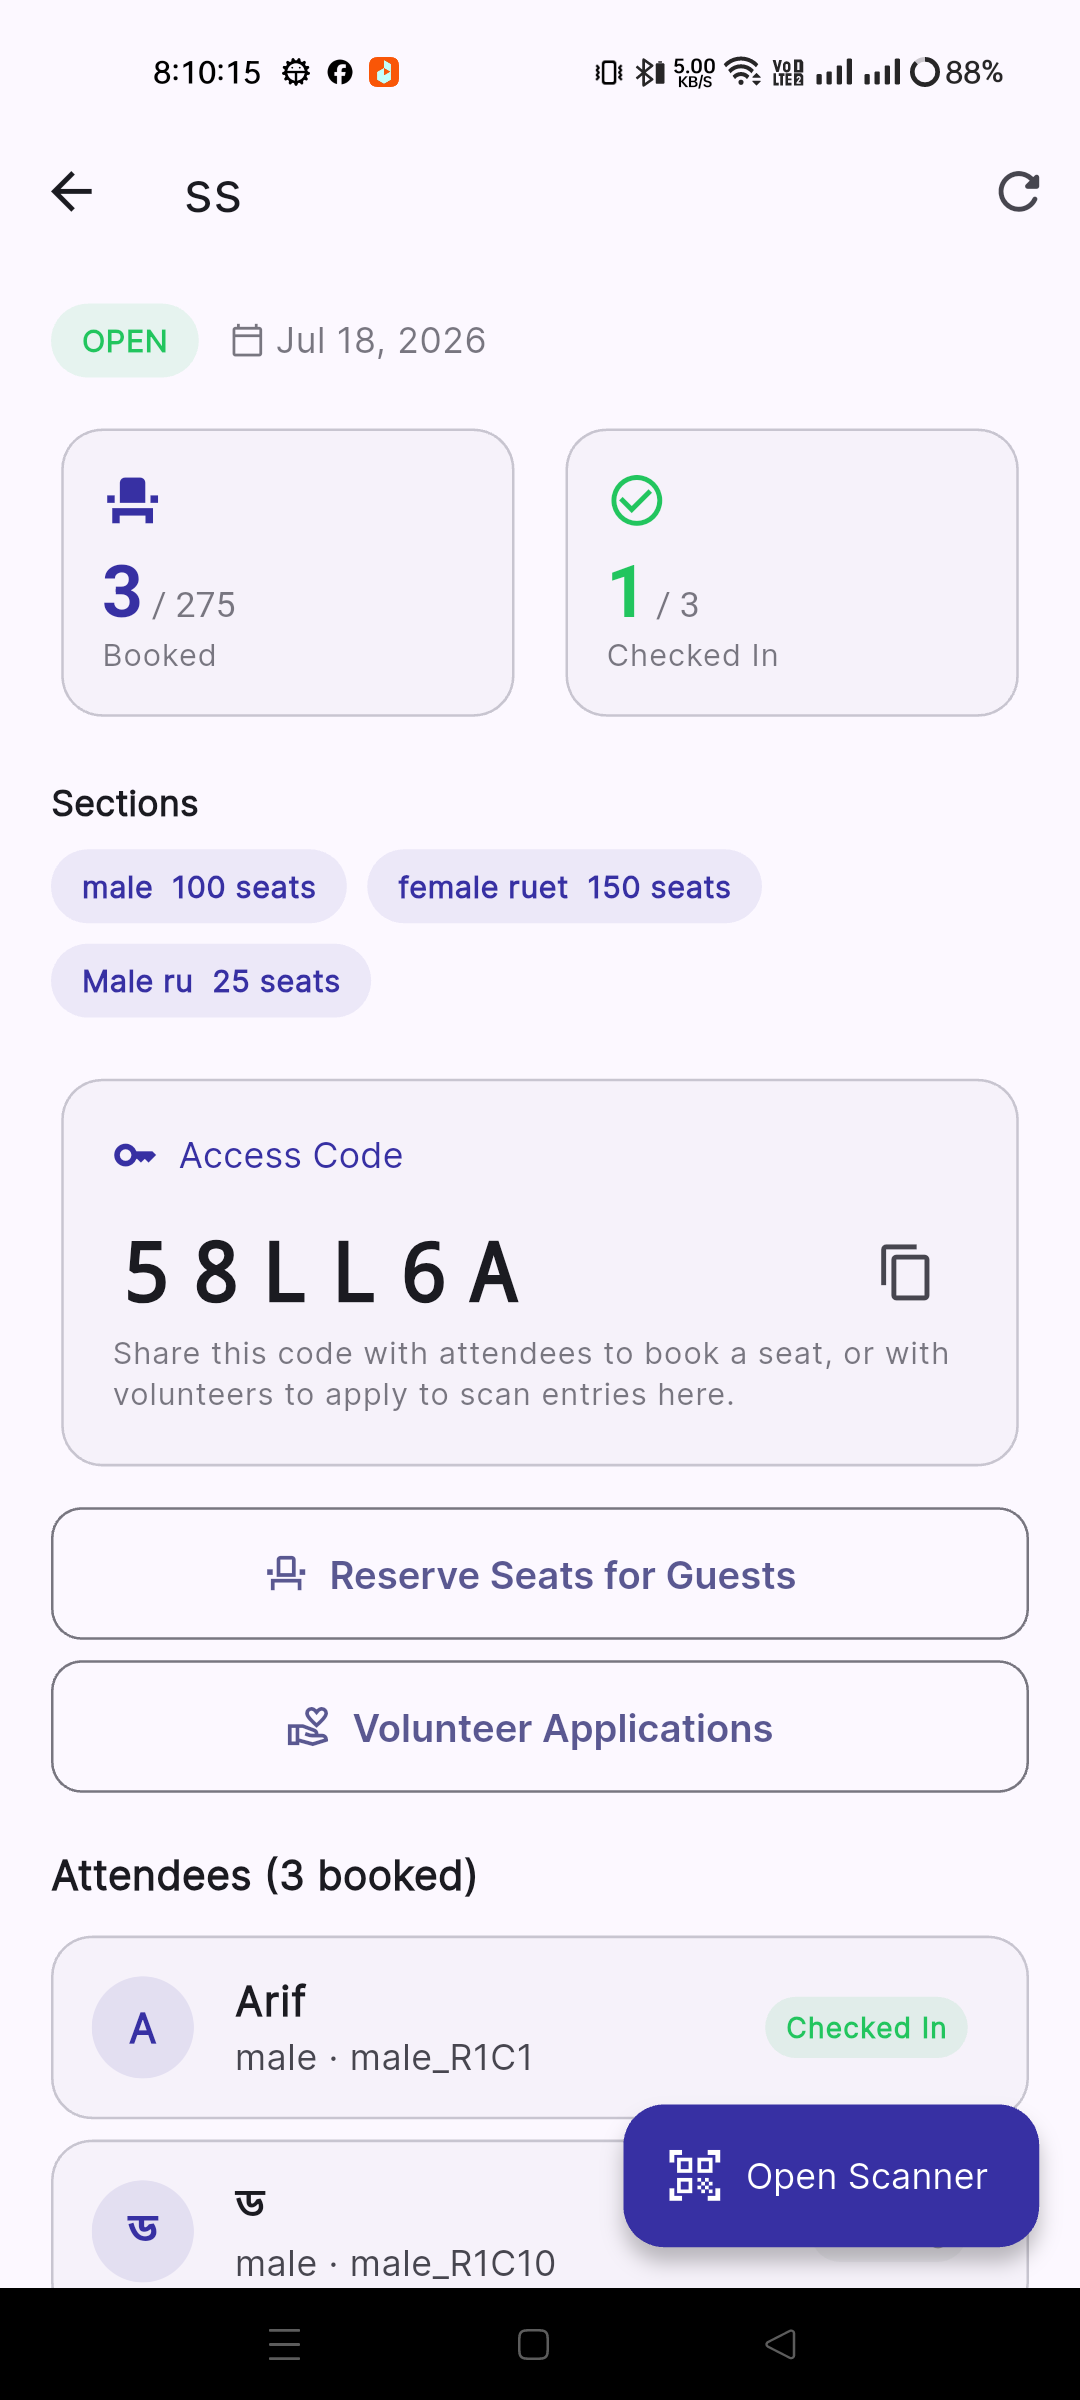
\includegraphics[width=0.42\textwidth]{screenshots/15_venue_detail_populated.png}
    \caption{A live venue with sections, bookings, and check-in status}
\end{figure}

\subsection{Reserving Seats for Guests}

\textbf{Reserve Seats for Guests} opens the admin seat map. Blue seats are
available, grey ones are already booked by attendees, and amber ones are
reserved by you. Tap an available seat, note who it is for, and confirm ---
that seat is then held back and cannot be booked by the public. Tapping a
reserved seat again releases it.

\begin{figure}[H]
    \centering
    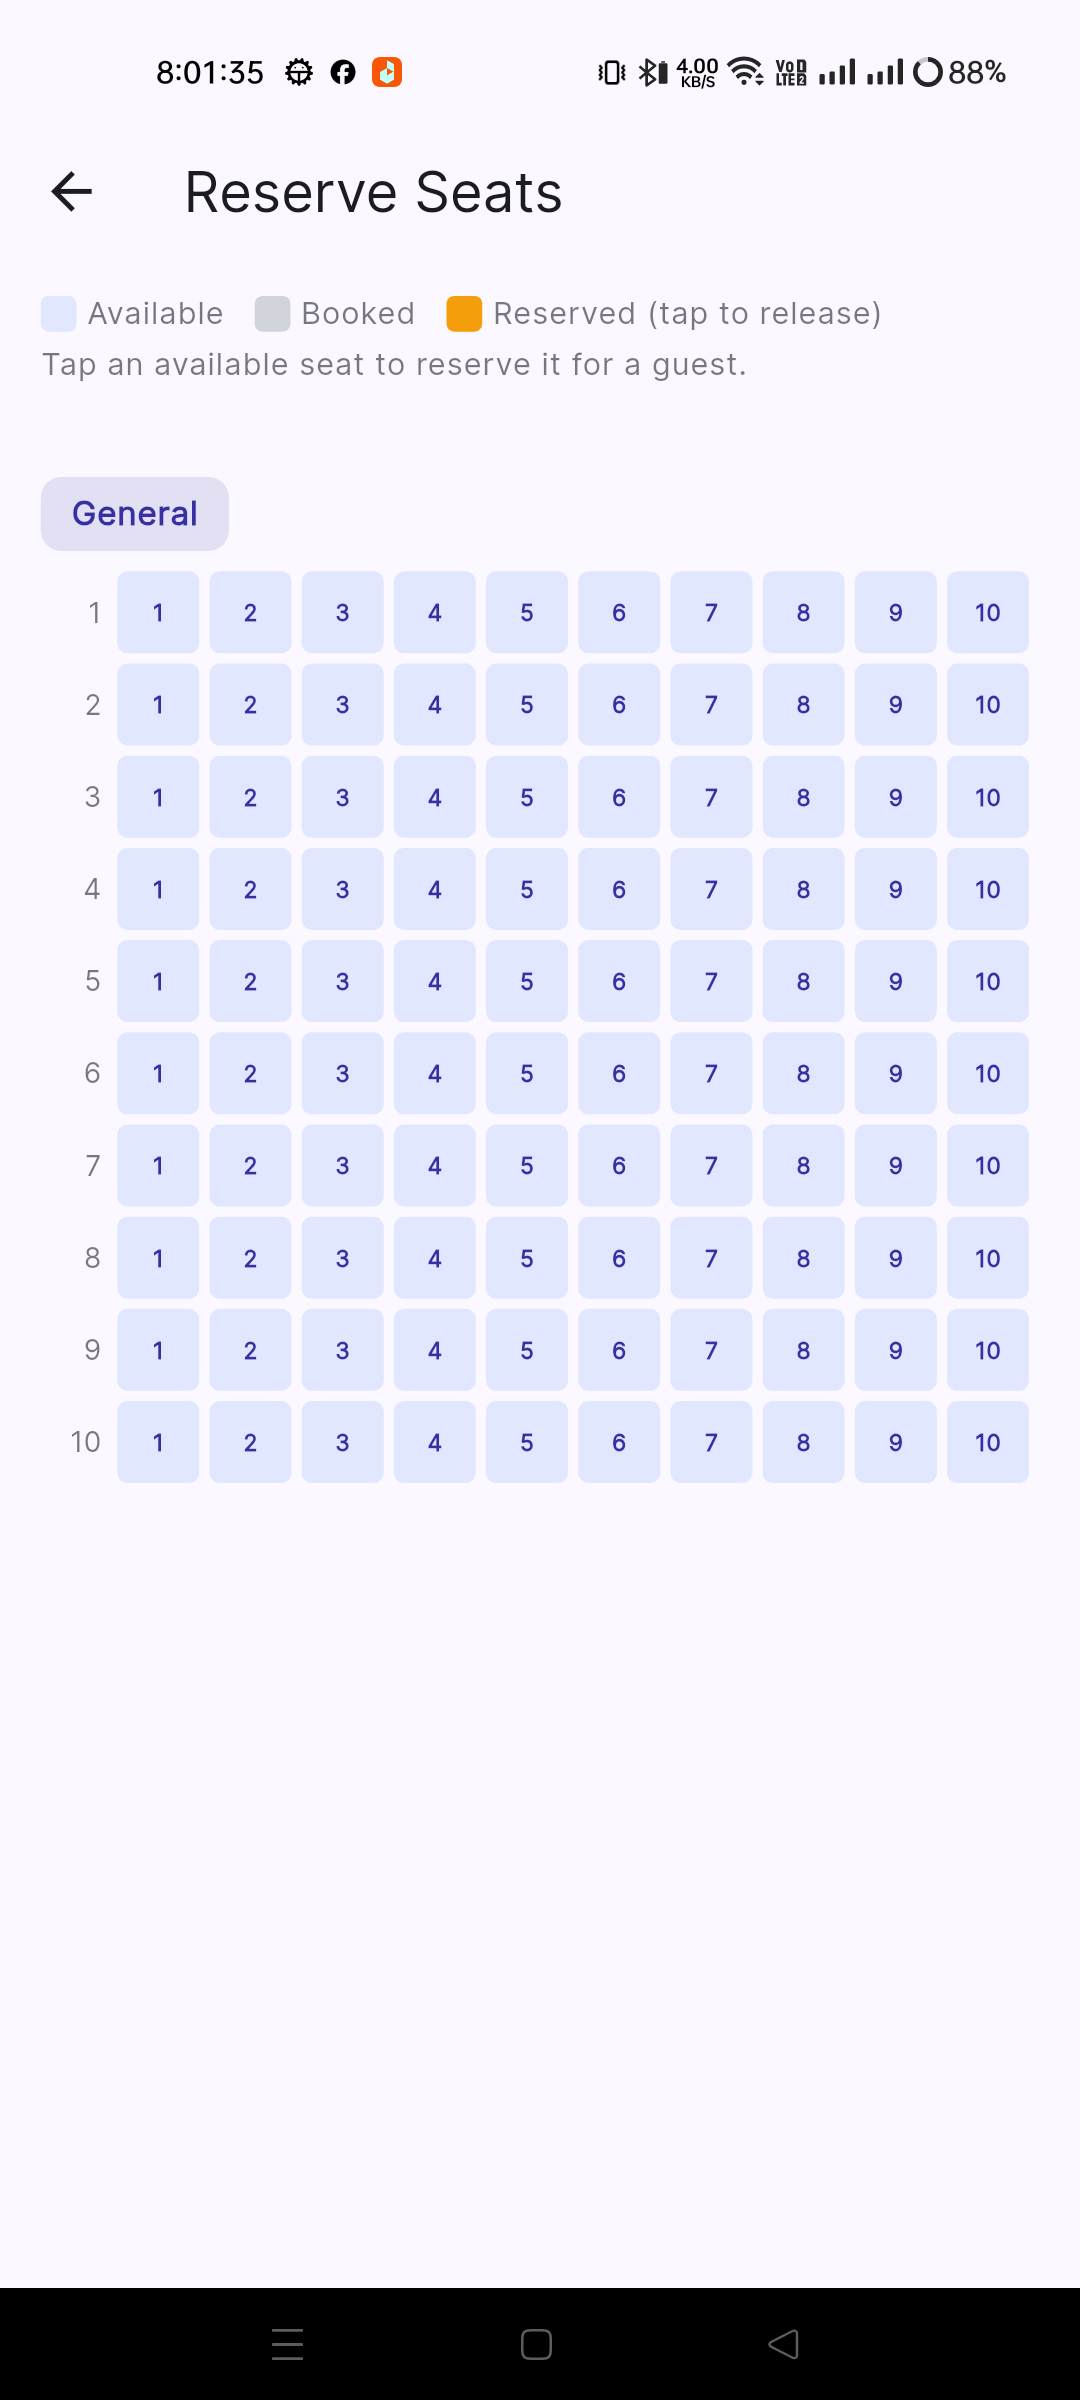
\includegraphics[width=0.42\textwidth]{screenshots/07_reserve_seats.png}
    \hfill
    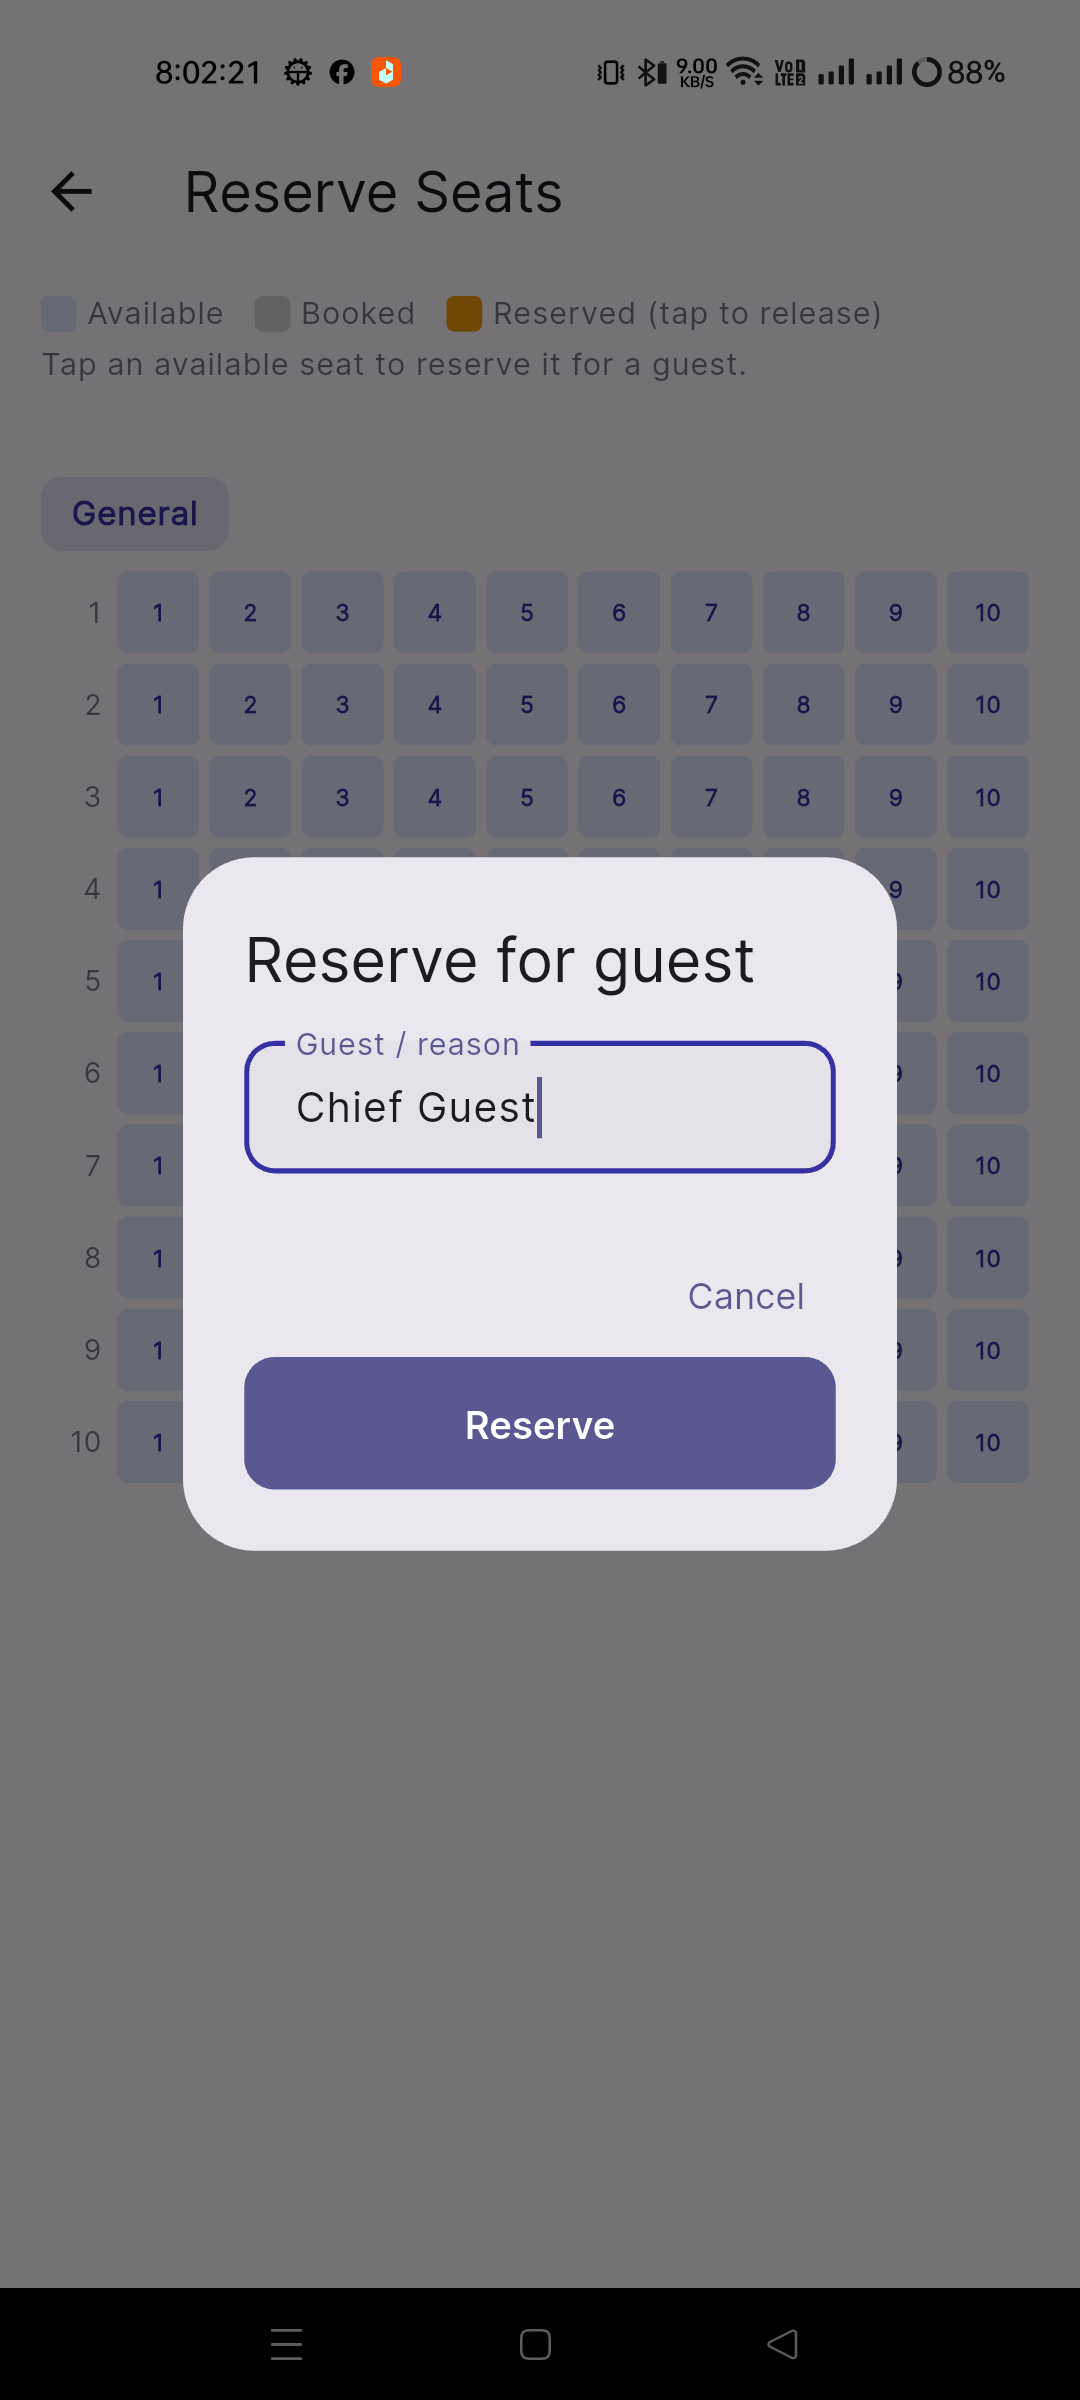
\includegraphics[width=0.42\textwidth]{screenshots/08_reserve_dialog.png}
    \caption{Left: the reservation seat map. Right: naming the guest.}
\end{figure}

\subsection{Approving Volunteers}

\textbf{Volunteer Applications} lists everyone who has applied to help at
this venue using its access code. Approving an applicant gives their device
--- and only their device --- permission to scan entry passes for this
venue; rejecting or revoking removes it again. Until an application is
approved, the volunteer cannot check anyone in.

\subsection{Checking People In}

\textbf{Open Scanner} turns the phone into a check-in station. The banner at
the top shows live progress (for example \textit{1 / 3 checked in}), the
camera window reads entry-pass QR codes, and the list underneath holds every
booked attendee. Point the camera at an attendee's pass to check them in
instantly, or use the \textbf{Check In} button beside a name to admit
someone manually if their screen is broken or their battery is dead.

\begin{figure}[H]
    \centering
    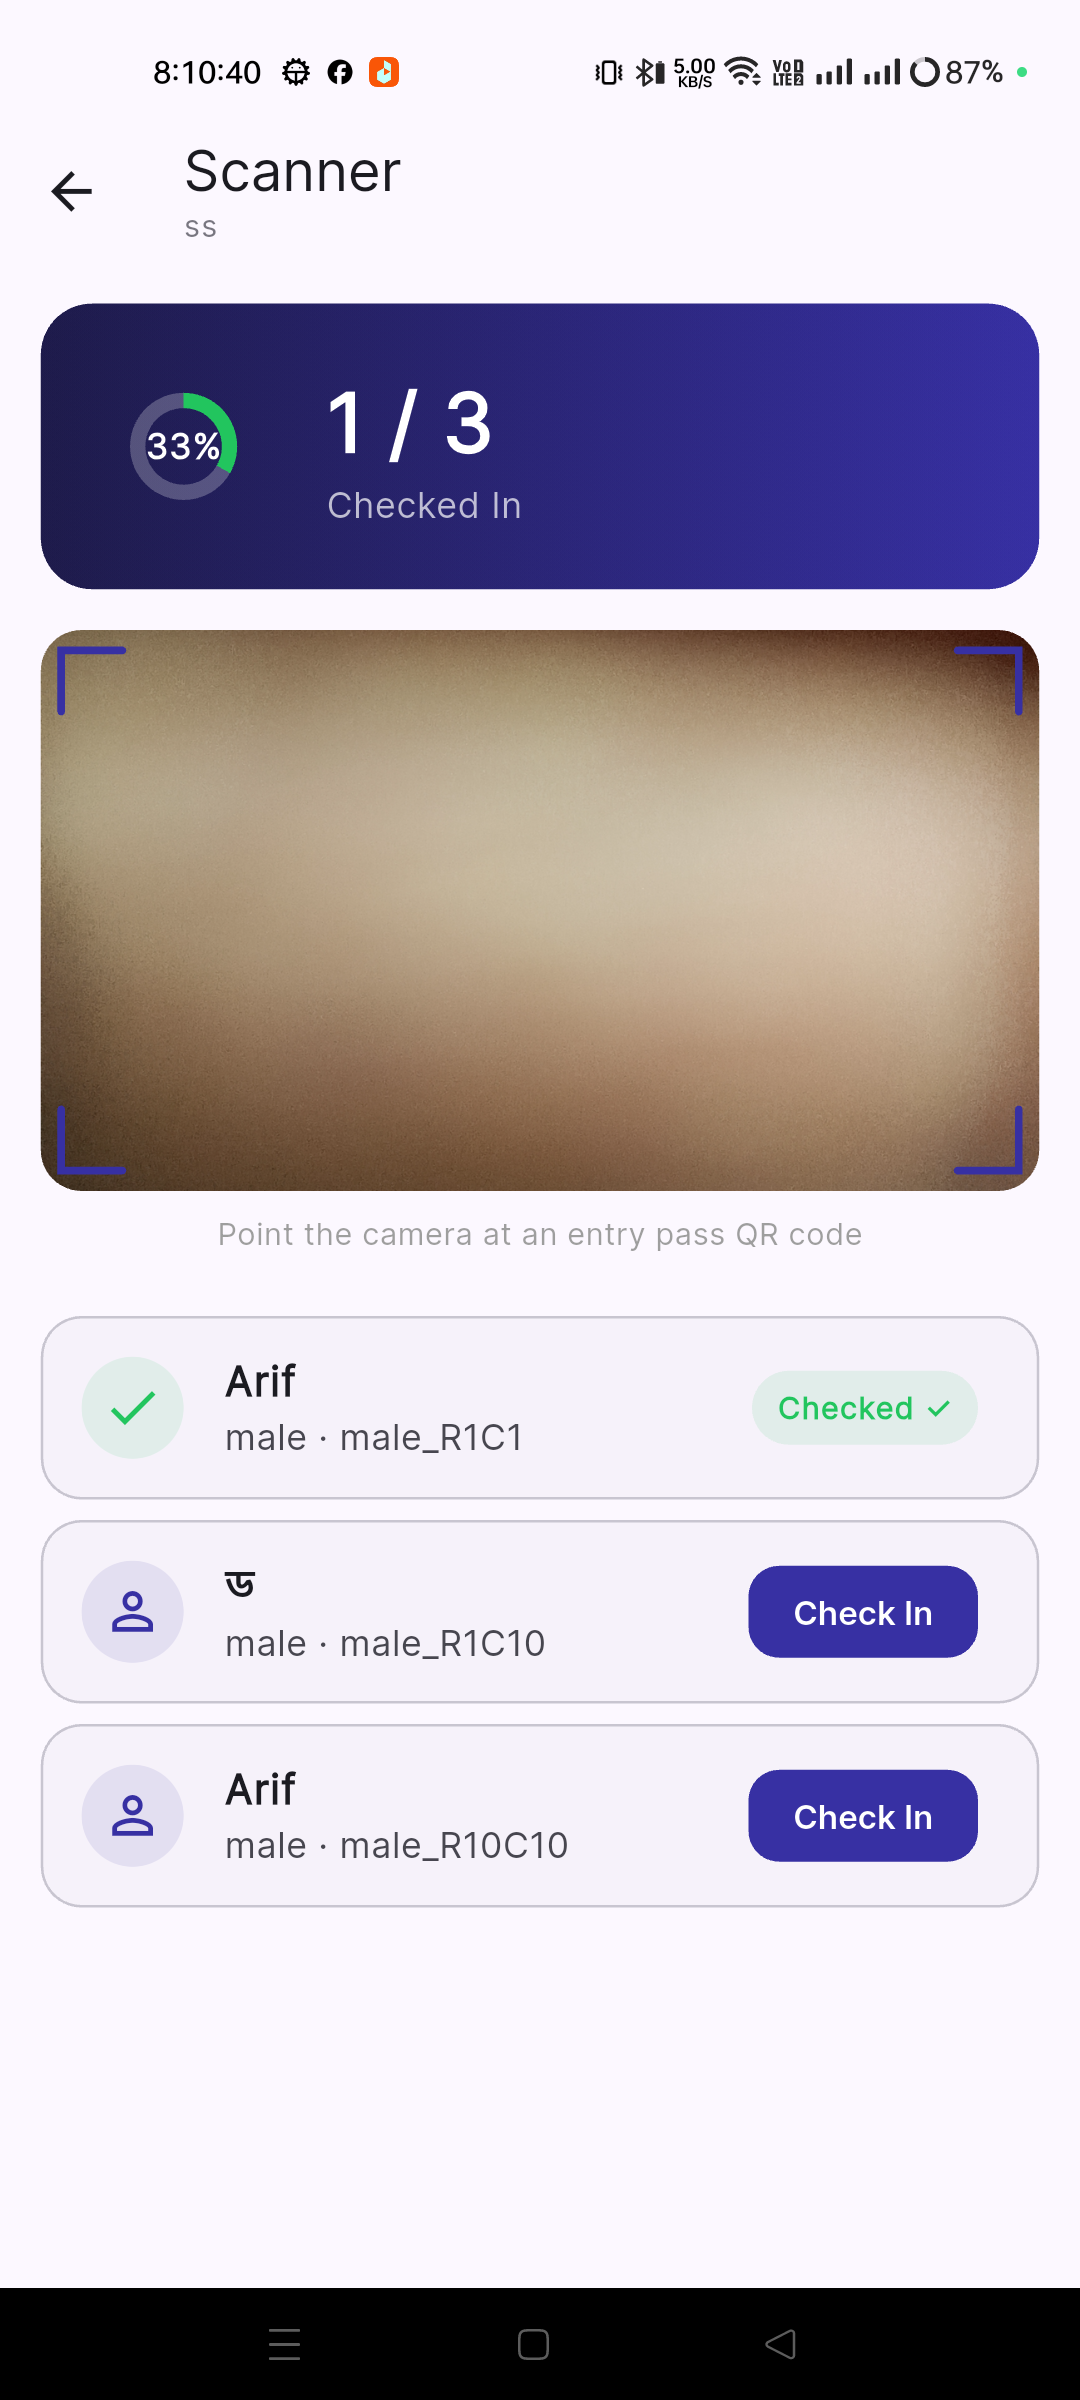
\includegraphics[width=0.42\textwidth]{screenshots/16_scanner.png}
    \caption{The scanner: live progress, camera, and manual check-in}
\end{figure}

% ─────────────────────────────────────────────────────────────
\section{For Attendees}

\subsection{Joining a Venue}

Choose \textbf{Audience} and enter the six-character code the organizer gave
you, then tap \textbf{Join Venue}. Passes you already hold are listed below
under \textbf{My Entry Passes}, so you can reopen them at any time --- even
without a network connection.

\begin{figure}[H]
    \centering
    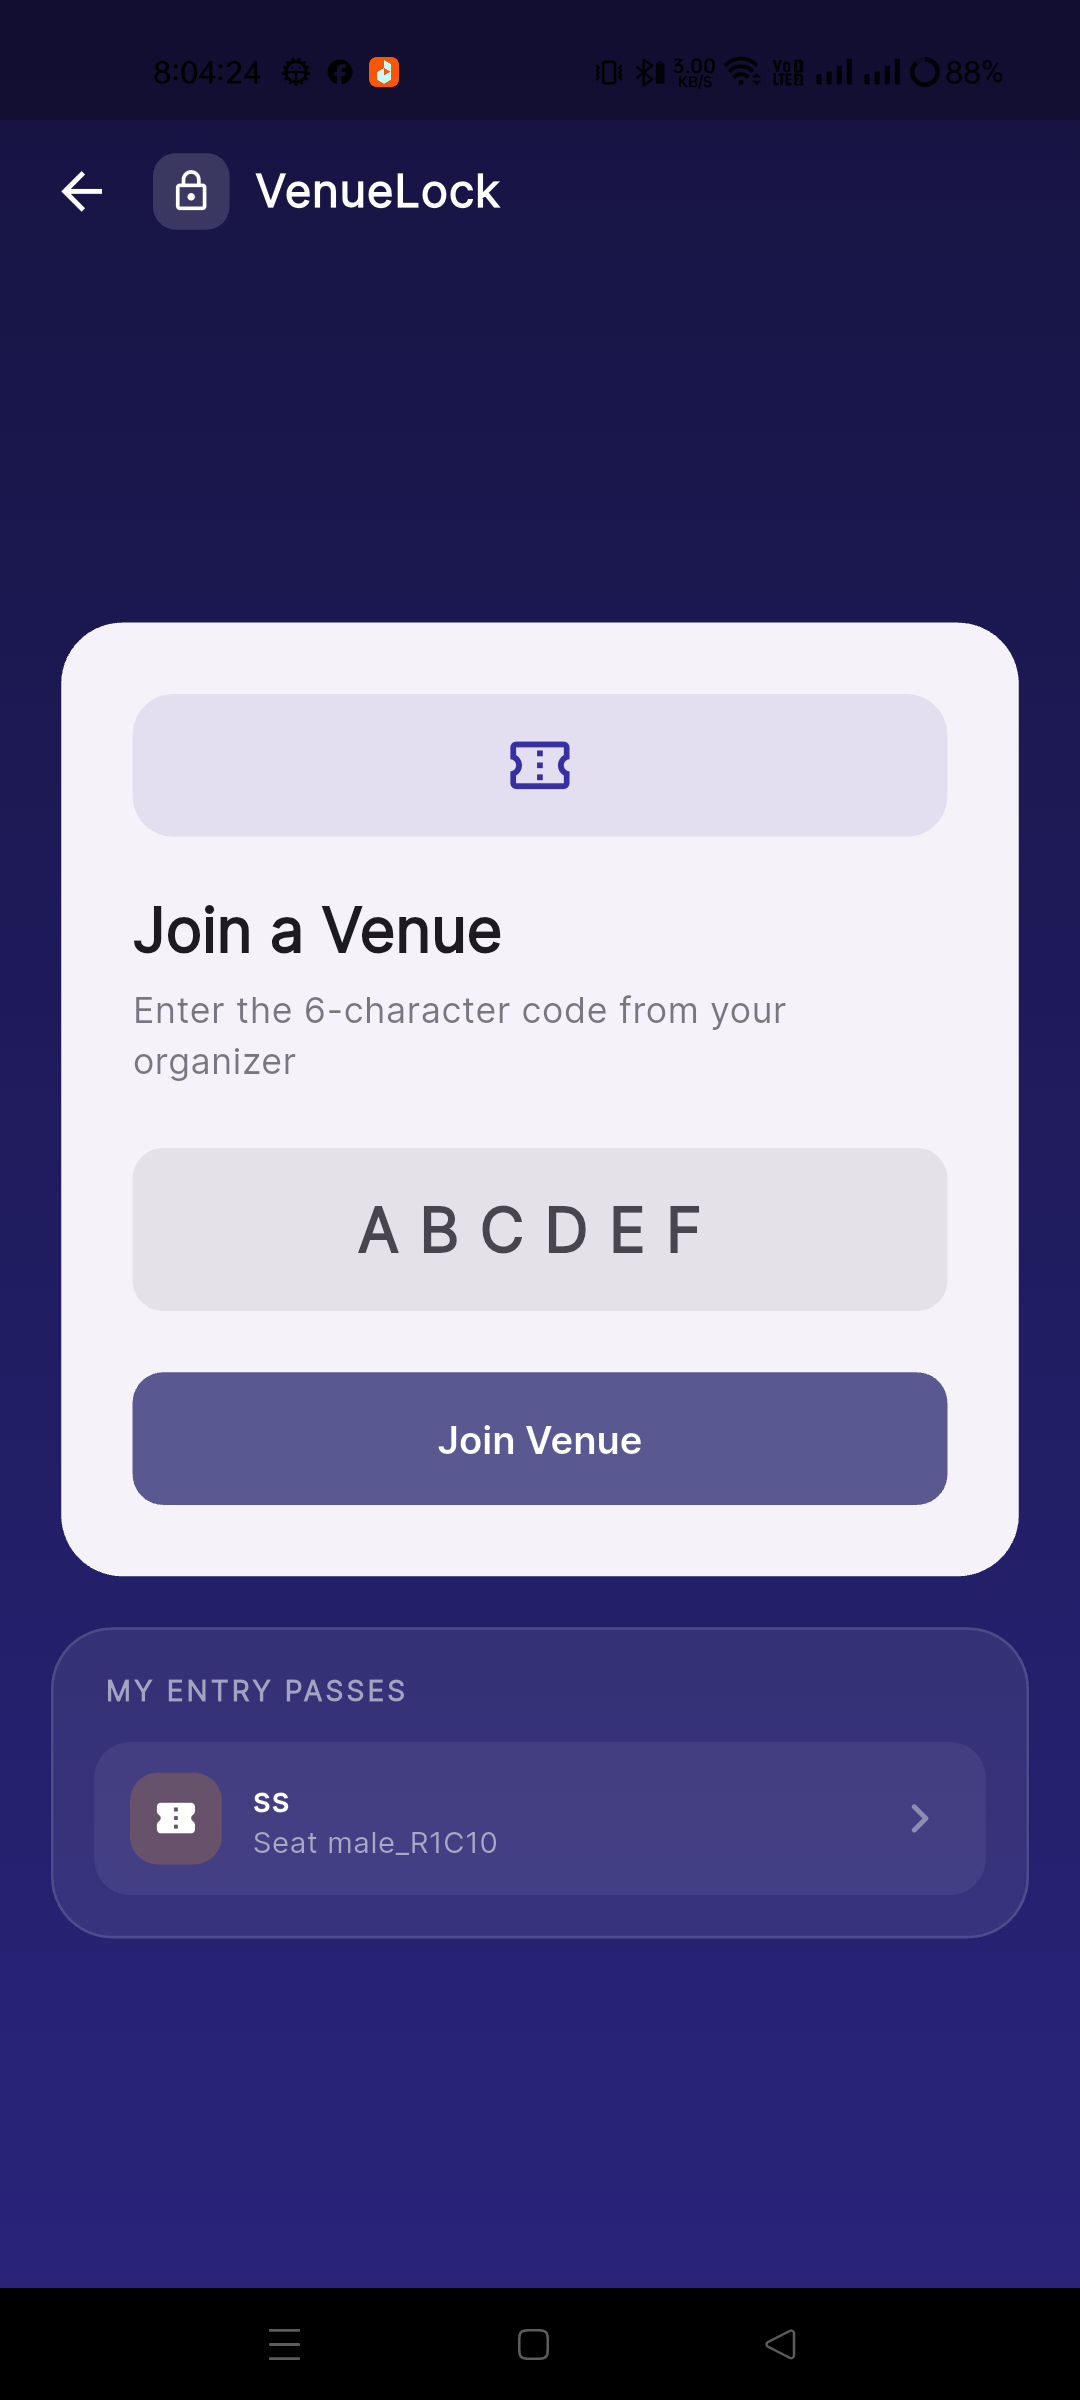
\includegraphics[width=0.42\textwidth]{screenshots/09_audience_join.png}
    \caption{Join a venue with its access code}
\end{figure}

\subsection{Picking a Seat}

The venue's live seat map opens. Blue seats are free, grey seats are taken.
If the venue has several sections, use the chips above the grid to switch
between them.

\begin{figure}[H]
    \centering
    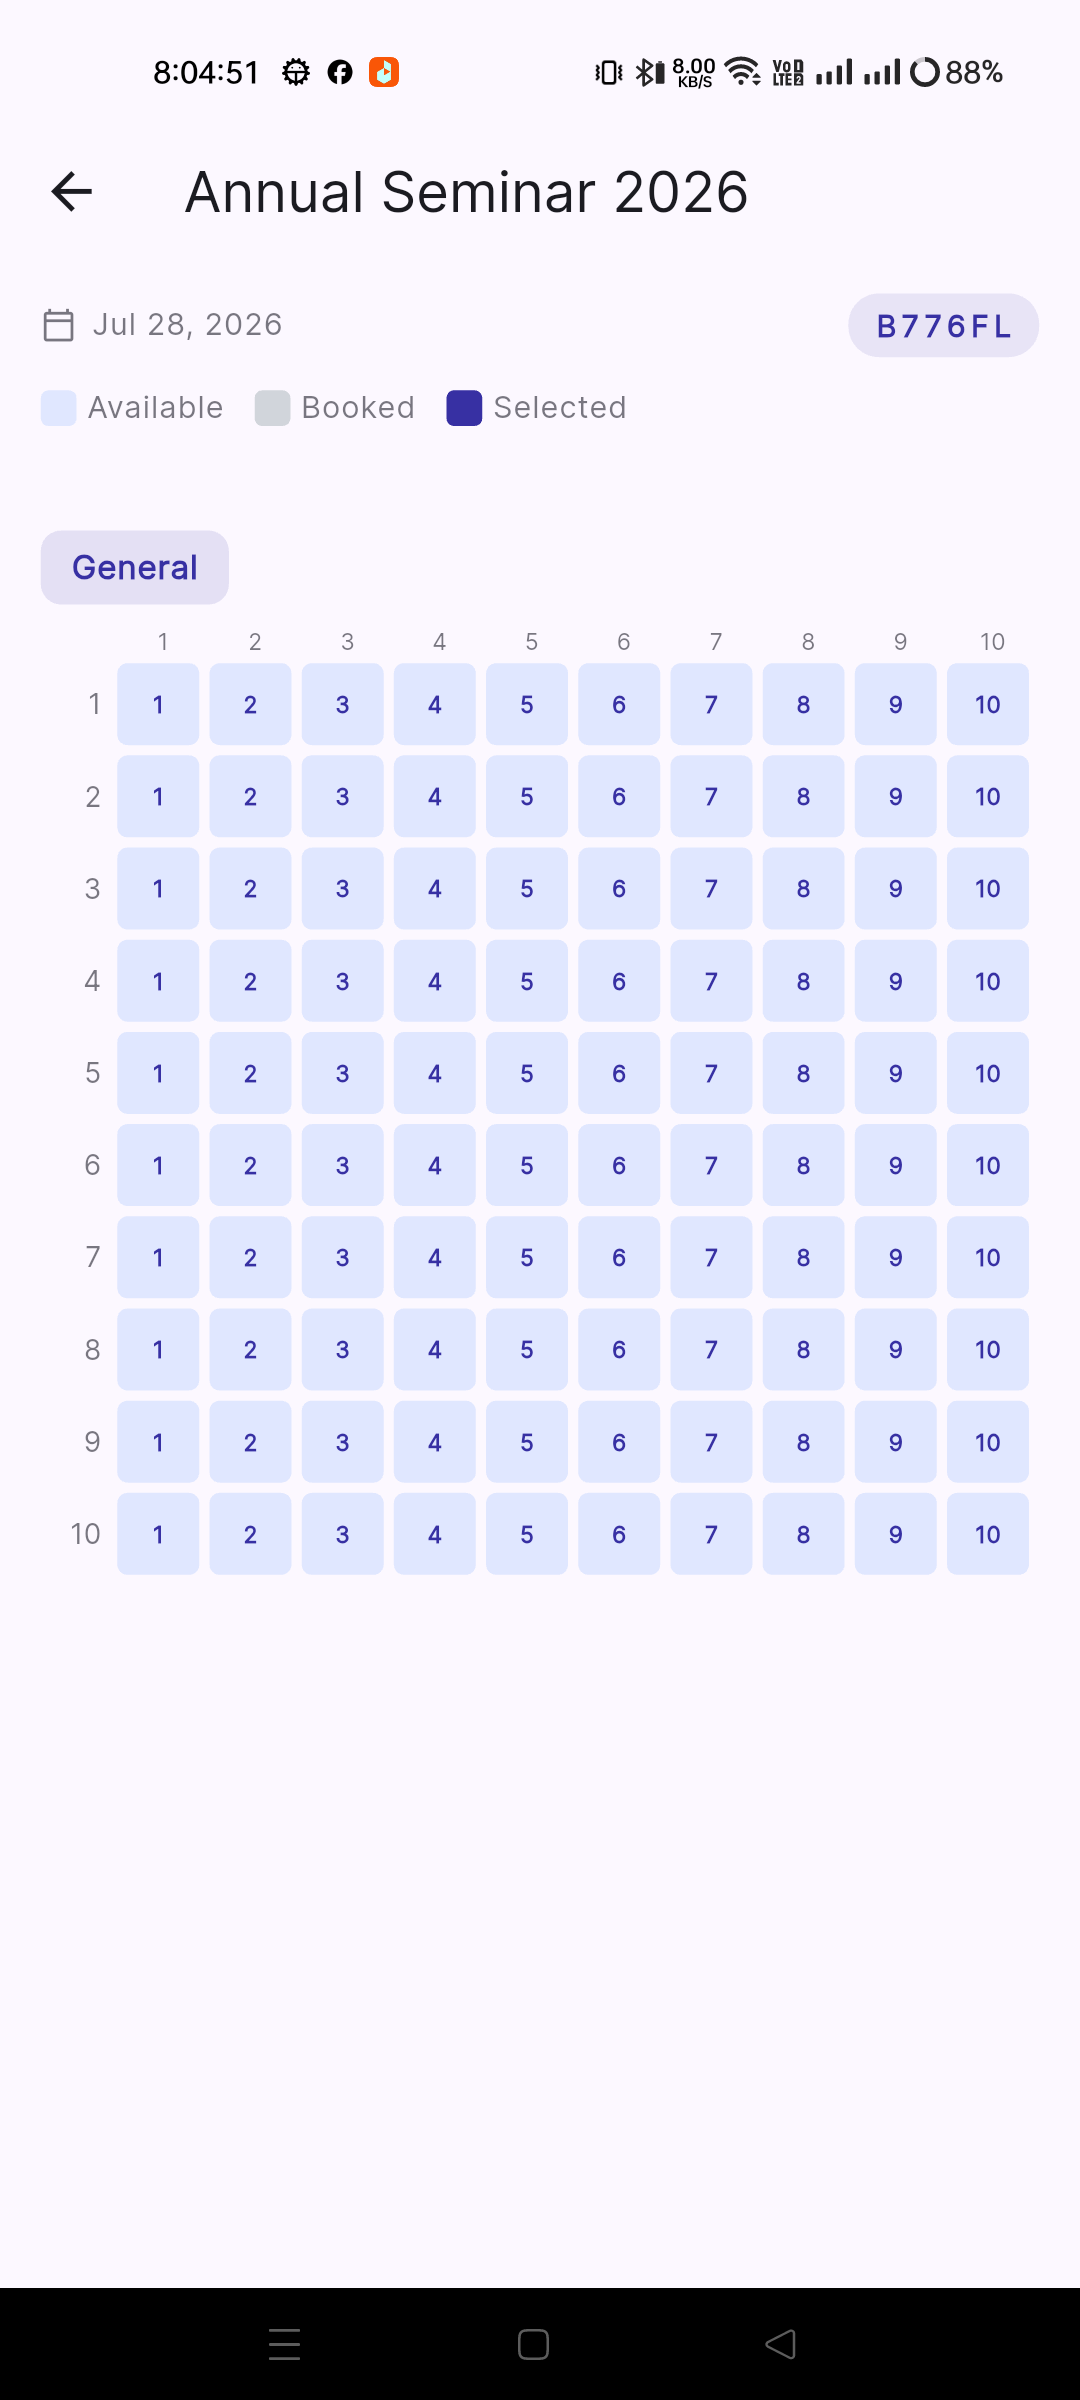
\includegraphics[width=0.42\textwidth]{screenshots/10_audience_seatmap.png}
    \hfill
    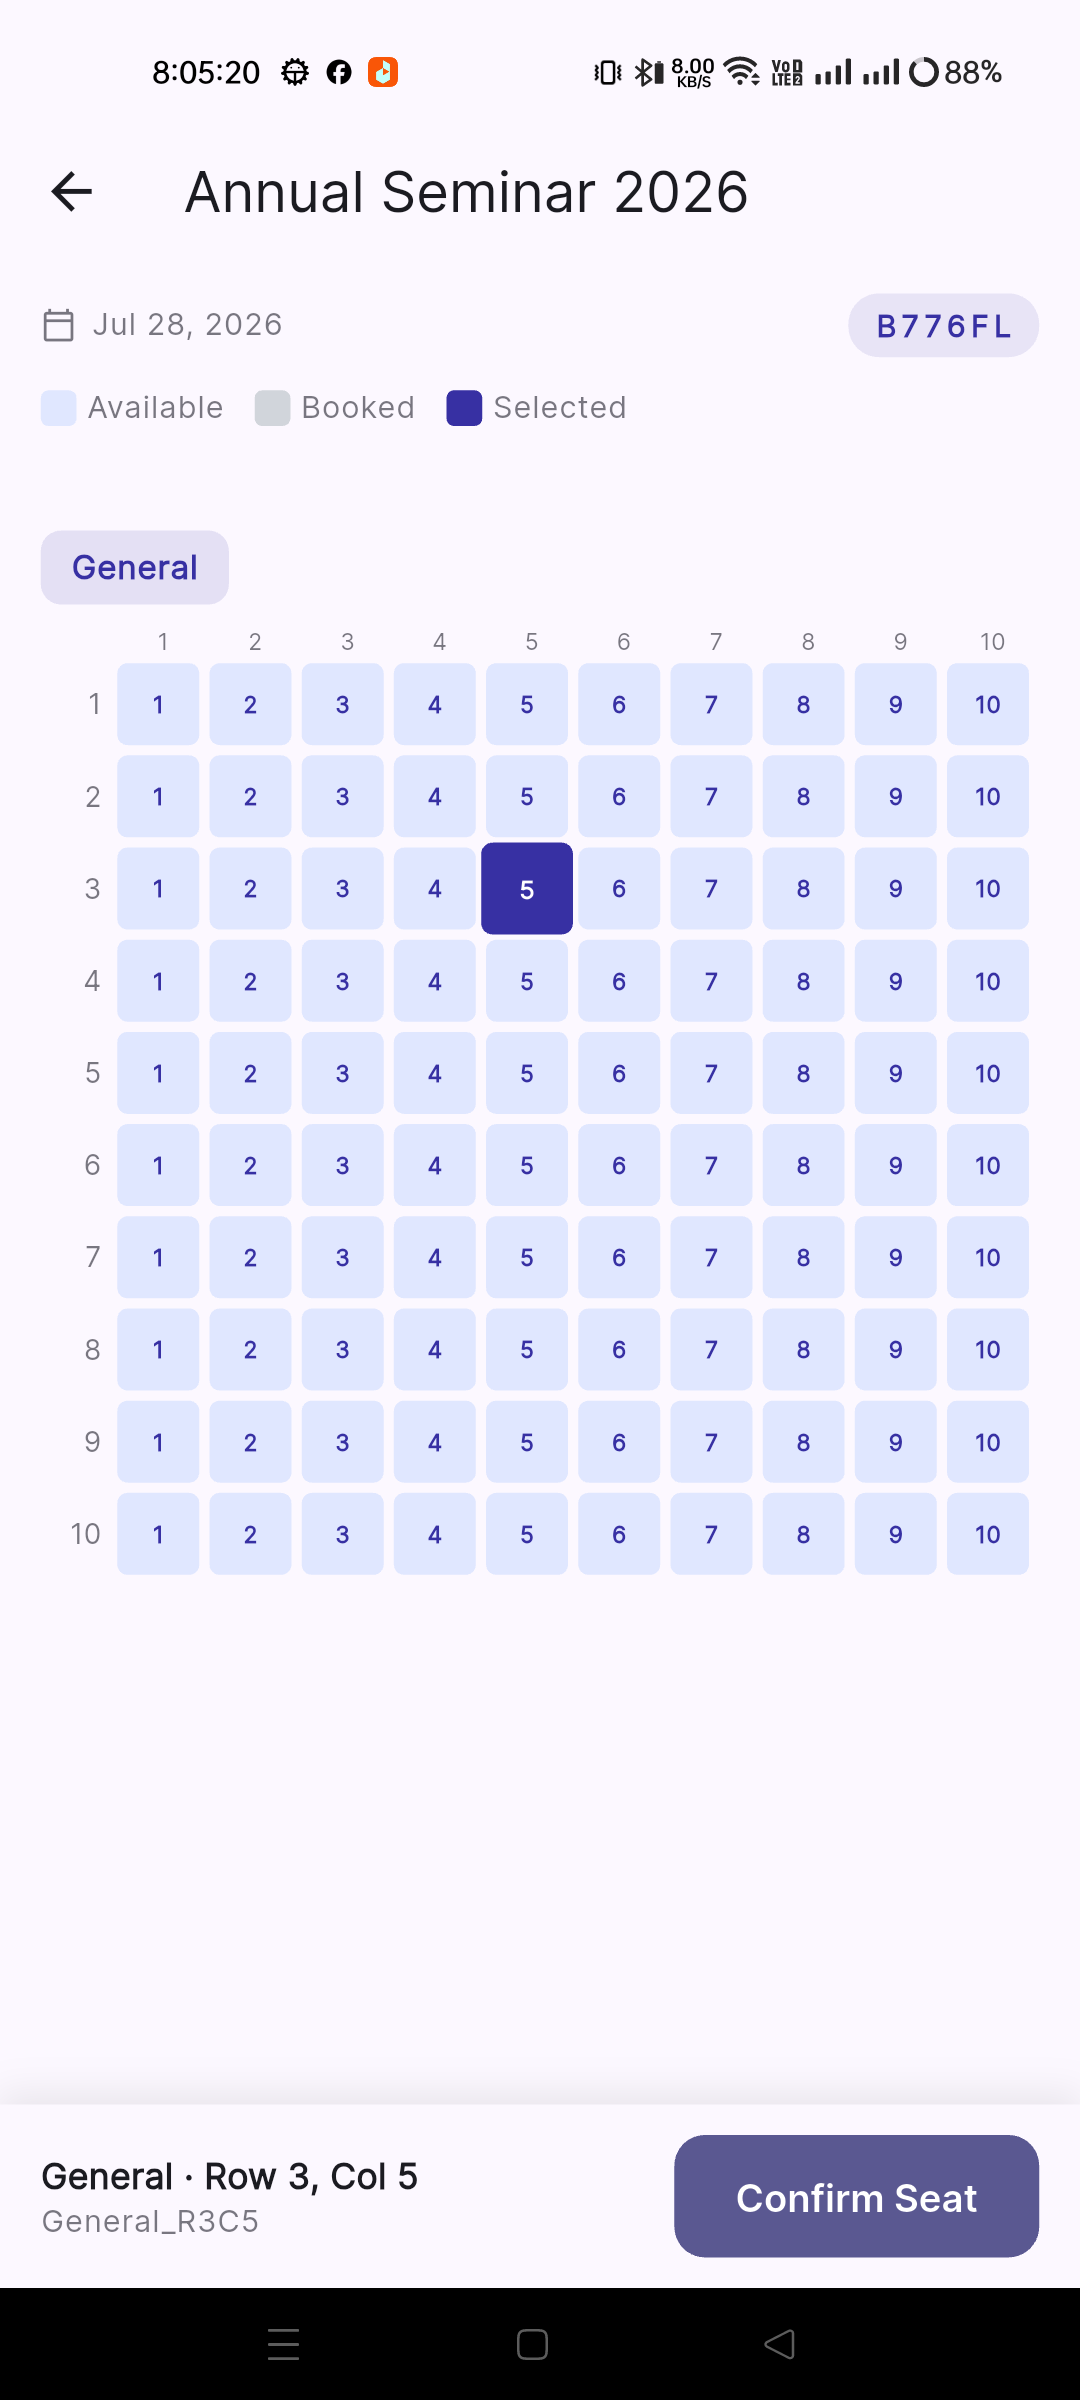
\includegraphics[width=0.42\textwidth]{screenshots/11_audience_seat_selected.png}
    \caption{Left: the live seat map. Right: a selected seat, ready to confirm.}
\end{figure}

Tap a free seat --- it turns dark blue and the bar at the bottom names it
(for example \textit{General $\cdot$ Row 3, Col 5}). Tap \textbf{Confirm
Seat} to continue.

\subsection{Booking Your Seat}

Fill in your name, email, and roll number, then tap \textbf{Book My Seat}.
If you have saved a profile, these fields are already filled in for you. The
seat is claimed on the server at this moment; if someone else took it in the
meantime, you will be asked to pick another.

\begin{figure}[H]
    \centering
    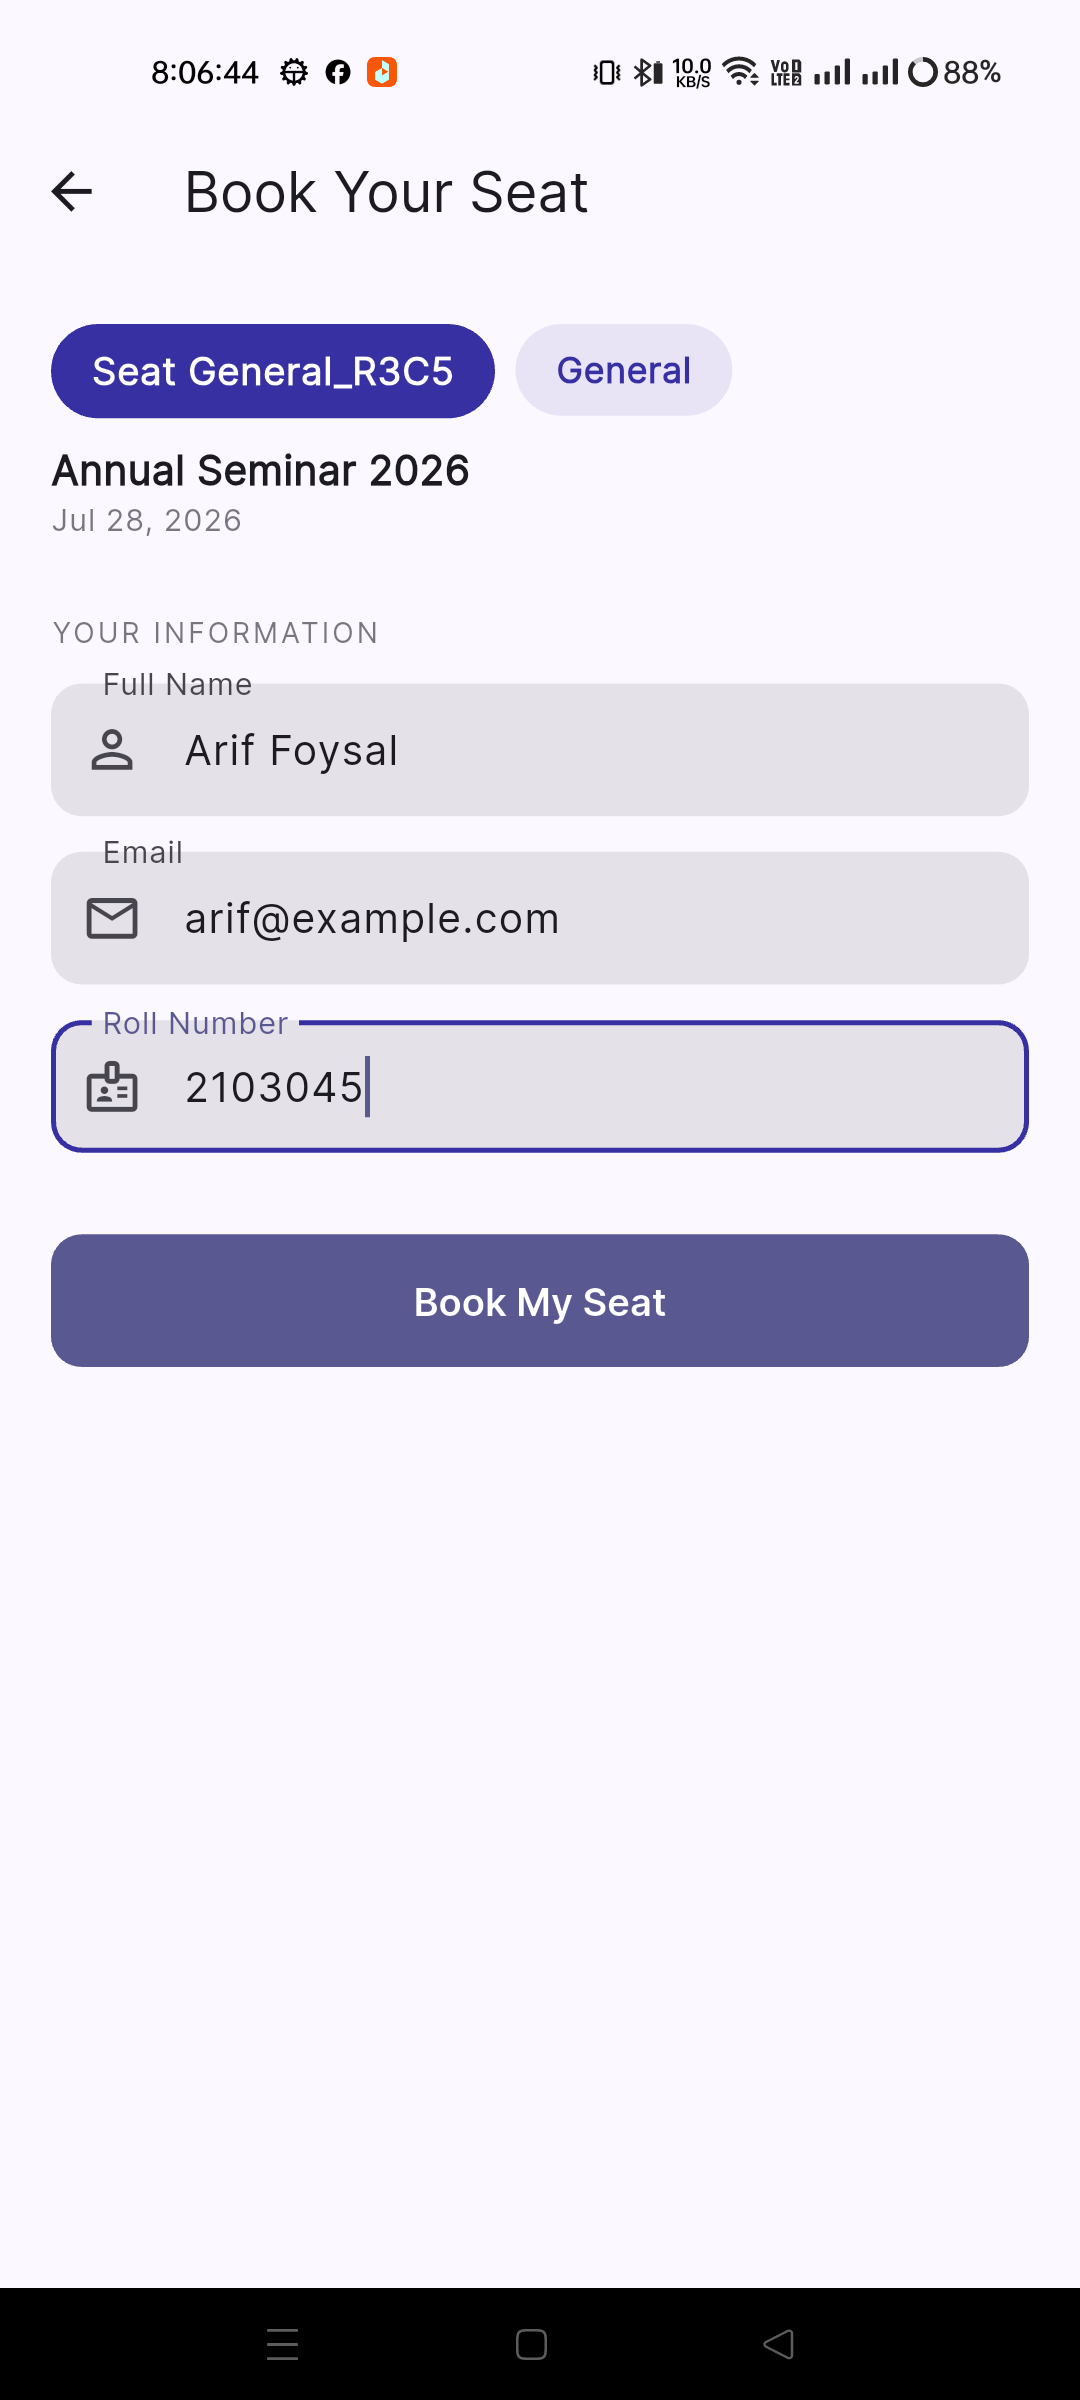
\includegraphics[width=0.42\textwidth]{screenshots/12_audience_booking_form.png}
    \caption{Confirm your details and book}
\end{figure}

\subsection{Your Entry Pass}

The booking produces your \textbf{entry pass}: a QR code with the venue
name, date, seat, section, and your details, marked \textbf{Valid Entry
Pass}. Show this at the door to be scanned in.

The pass is stored on your phone, so it opens again from \textbf{My Entry
Passes} even after the app is closed. Use \textbf{Save} to keep a copy in
your gallery, or \textbf{Share} to send it to yourself as a backup.

\begin{figure}[H]
    \centering
    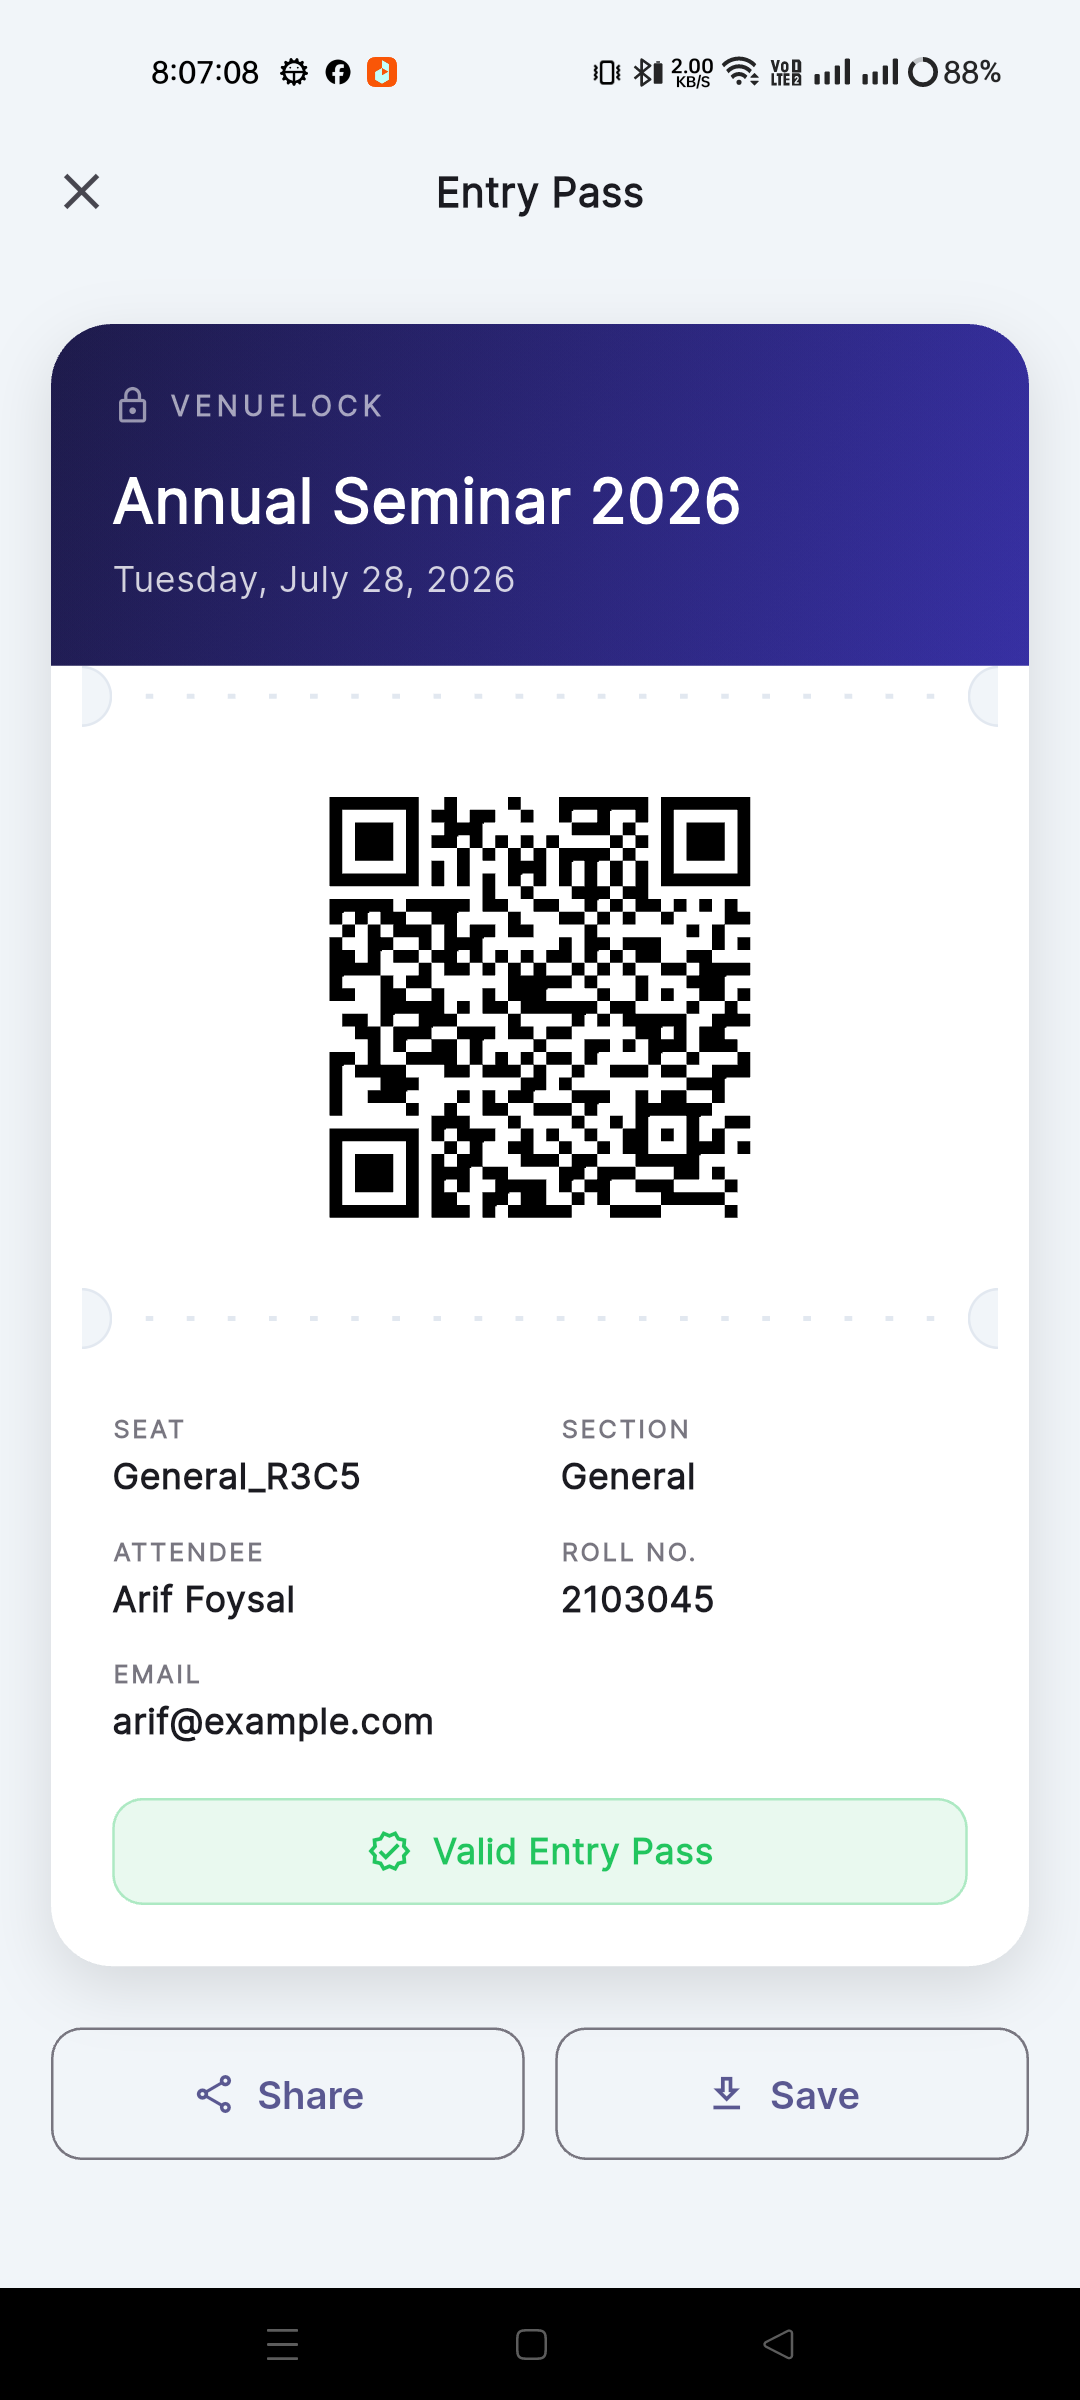
\includegraphics[width=0.42\textwidth]{screenshots/13_entry_pass.png}
    \caption{A QR entry pass}
\end{figure}

% ─────────────────────────────────────────────────────────────
\section{For Volunteers}

Choose \textbf{Volunteer}, enter the venue's access code and your name (a
phone number is optional), and tap \textbf{Apply}. The organizer sees your
application on their Volunteer Applications screen.

\begin{figure}[H]
    \centering
    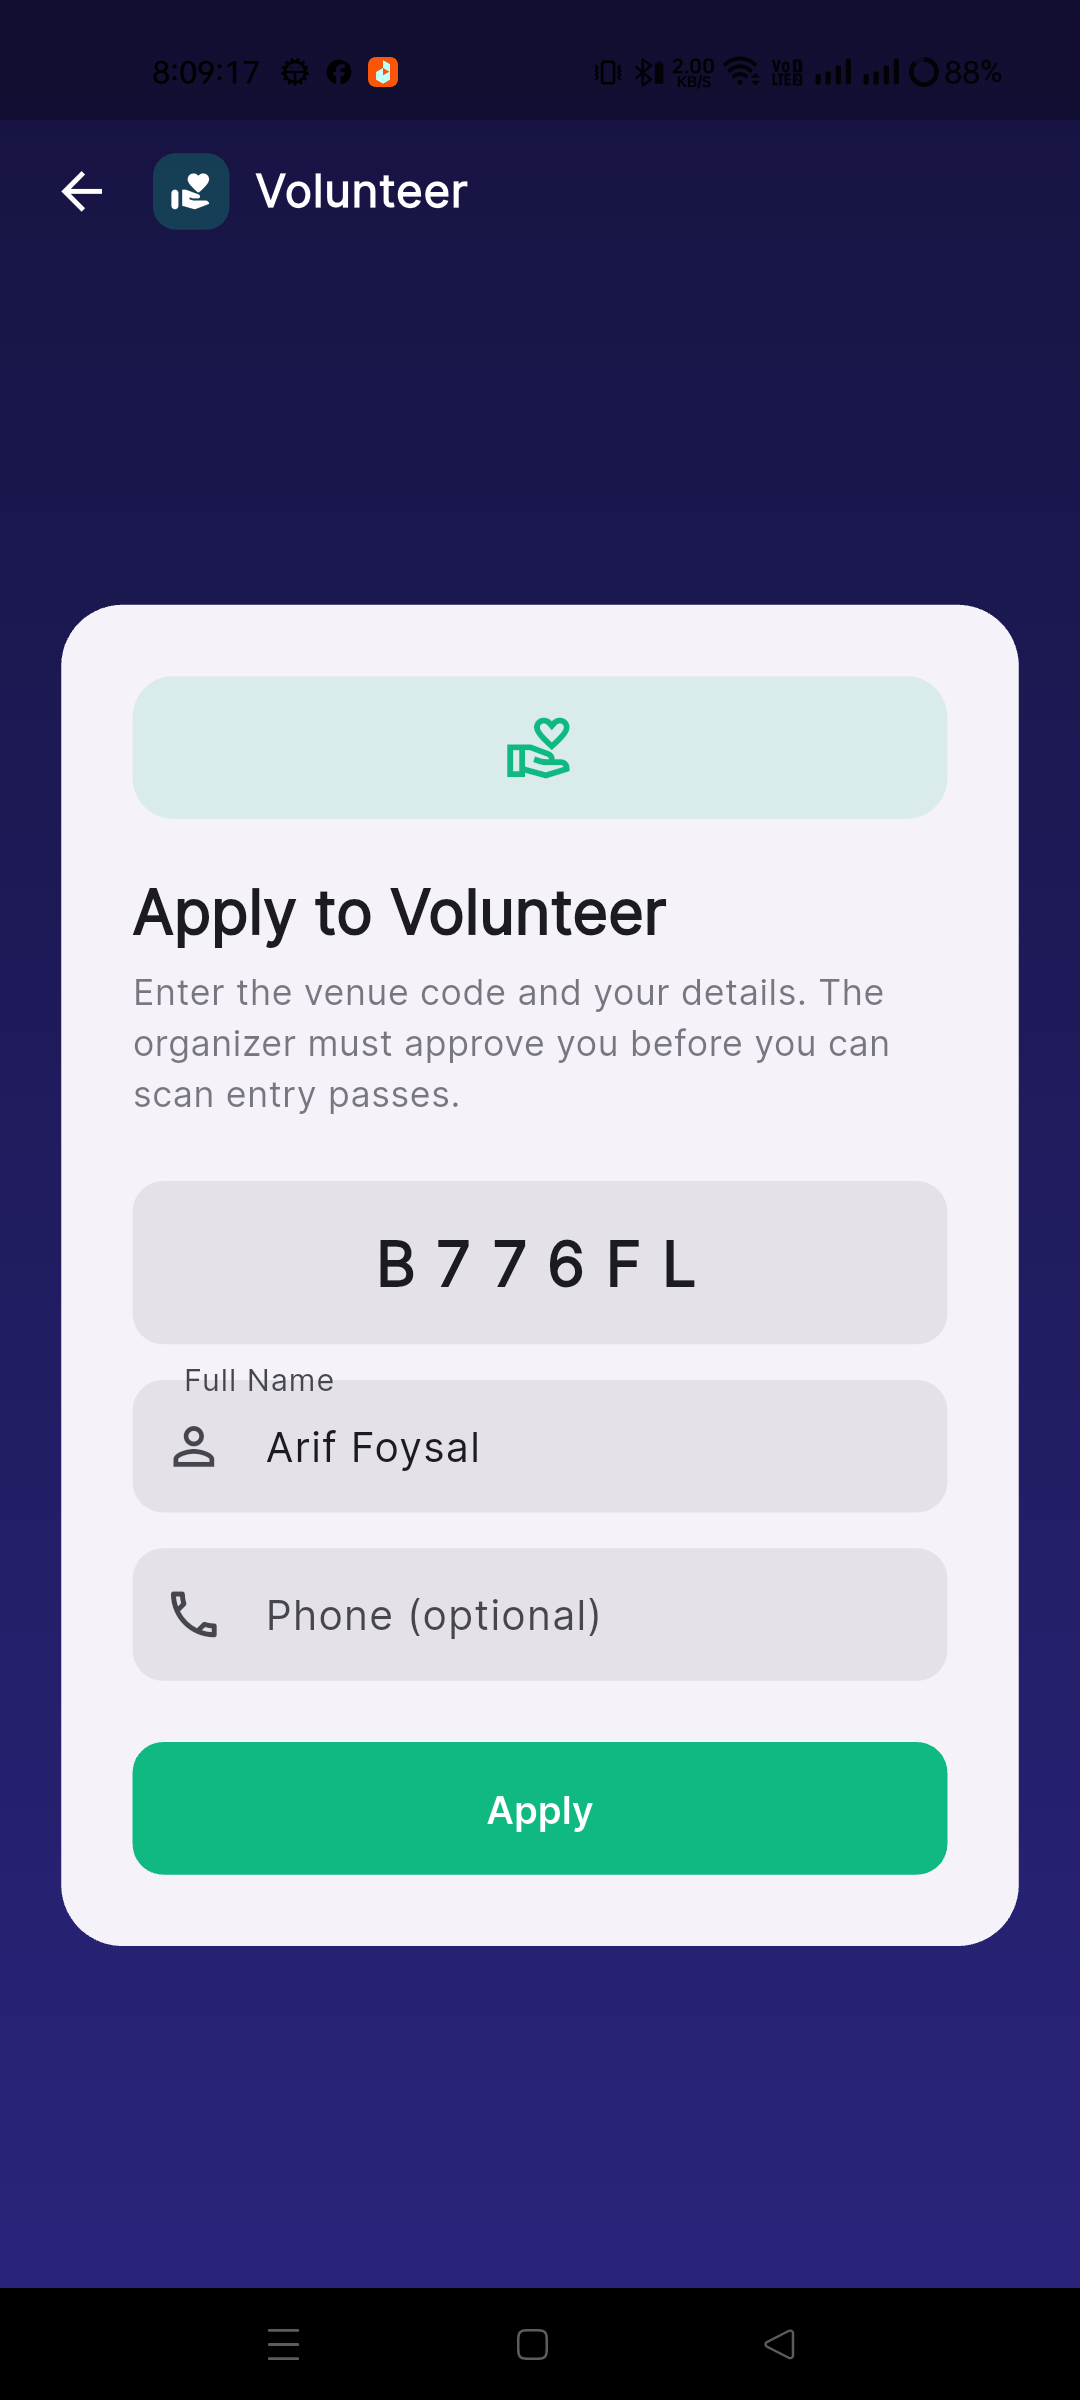
\includegraphics[width=0.42\textwidth]{screenshots/14_volunteer_apply.png}
    \caption{Applying to volunteer at a venue}
\end{figure}

Once the organizer approves you, the scanner unlocks on your device and you
can check attendees in exactly as described in
\textit{Checking People In}. Your access is scoped to that one venue and to
the device you applied from --- there is no shared admin login to pass
around at the gate.

% ─────────────────────────────────────────────────────────────
\section{Tips and Troubleshooting}

\begin{itemize}[leftmargin=1.5em]
    \item \textbf{The code is not working.} Access codes are six characters
        and are not case-sensitive; check for a confused \texttt{0} and
        \texttt{O}. Make sure the organizer has published the venue.
    \item \textbf{My seat was taken while I was booking.} Seat ownership is
        decided by the server at the moment you tap \textbf{Book My Seat},
        so a busy venue can lose you a seat between selecting and
        confirming. Pick another free seat and try again.
    \item \textbf{The scanner shows a black window.} VenueLock needs
        camera permission. Grant it in Android
        \textit{Settings $\rightarrow$ Apps $\rightarrow$ VenueLock $\rightarrow$
        Permissions}, then reopen the scanner.
    \item \textbf{An attendee's phone is dead.} Find their name in the
        scanner's attendee list and use the \textbf{Check In} button to
        admit them manually.
    \item \textbf{Counts look out of date.} The venue screen refreshes on a
        timer; the refresh icon in the top-right corner forces an immediate
        update.
    \item \textbf{Keep guest seats out of the public pool.} Reserve them
        from the admin seat map \emph{before} you share the access code.
\end{itemize}

% ─────────────────────────────────────────────────────────────
\section{Where to Get VenueLock}

\begin{itemize}[leftmargin=1.5em]
    \item Web app and landing page:
        \url{https://theobsidianeye-arif-foysal.github.io/Venue-Lock-v1/}
    \item Android APK:
        \url{https://github.com/TheObsidianEye-ARIF-FOYSAL/Venue-Lock-v1/releases/latest/download/VenueLock.apk}
    \item Source code:
        \url{https://github.com/TheObsidianEye-ARIF-FOYSAL/Venue-Lock-v1}
\end{itemize}

\end{document}
